\documentclass[journal]{IEEEtran}

% *** CITATION PACKAGES ***
\usepackage{cite}

% *** GRAPHICS RELATED PACKAGES ***
\usepackage{multirow,makecell}
\usepackage{booktabs,pifont}
\newcolumntype{C}[1]{>{\centering\arraybackslash}m{#1}}
\newcolumntype{L}[1]{m{#1}}
\ifCLASSINFOpdf
  \usepackage[pdftex]{graphicx}
\else
\fi

% *** MATH PACKAGES ***
\usepackage{amsmath}
\usepackage{amssymb}

% *** ALGORITHM PACKAGES ***
\usepackage{algorithm}
\usepackage{algpseudocode}

% *** ALIGNMENT PACKAGES ***
\usepackage{array}

% *** SUBFIGURE PACKAGES ***
\usepackage{subfigure}

% *** URL PACKAGES ***
\usepackage{url}
\usepackage{orcidlink}

% *** TIKZ PACKAGES ***
\usepackage{tikz}
\usetikzlibrary{positioning,shapes,arrows.meta}

% ========================================================
%  H-ST-MBAN: Hybrid Spatio-Temporal Multi-Branch Attention Network
%  for RSU Dwell Time Prediction in CCVN
%  Target: IEEE Internet of Things Journal
% ========================================================

\begin{document}

\title{Deterministic RSU Dwell Time Prediction via\\Hybrid Multi-Branch Attention Network in Content-Centric Vehicular Networks}

\newcommand{\orcidauthorA}{0000-0003-3971-0715} % Youngju Nam
\newcommand{\orcidauthorB}{0000-0001-8209-5944} % Jeong-Hun Kim
\newcommand{\orcidauthorC}{0000-0002-0422-0647} % Euisin Lee

\author{Youngju Nam,~\IEEEmembership{Student Member,~IEEE,}
        Jeong-Hun Kim,~\IEEEmembership{Member,~IEEE,}
        and Euisin Lee,~\IEEEmembership{Member,~IEEE}

\thanks{Manuscript received April 00, 2026; revised August 00, 2026.
This work was supported by the National Research Foundation of Korea (NRF) grant funded by the Korean government Ministry of Science and ICT (MSIT) under Grant No. 2022R1A2C1010121.
\textit{(Corresponding author: Euisin Lee.)}}
\thanks{Youngju Nam is with the School of Software, Kunsan National University,
Gunsan 54150, Republic of Korea (e-mail: imnyj@kunsan.ac.kr).}
\thanks{Jeong-Hun Kim is with the Department of Computer Science and Information Engineering,
Kunsan National University, Gunsan 54150, Republic of Korea (e-mail: kimjh@kunsan.ac.kr).}
\thanks{Euisin Lee is with the School of Information and Communication Engineering,
Chungbuk National University, Cheongju 28644, Republic of Korea (e-mail: eslee@chungbuk.ac.kr).}
\thanks{Digital Object Identifier 10.0000/JIOT.2026.0000000}}

\markboth{IEEE Internet of Things Journal,~Vol.~00, No.~0, 2026}%
{Y. Nam \MakeLowercase{\textit{et al.}}: Deterministic RSU Dwell Time Prediction via Hybrid Multi-Branch Attention Network in CCVNs}

\IEEEpubid{2327-4662 \copyright~2026 IEEE}

\maketitle

% ============================================================
\begin{abstract}
In Content-Centric Vehicular Networks (CCVNs), proactive RSU caching requires accurate prediction of vehicle dwell time at the moment a content request is issued.
Prior work on vehicular mobility prediction relies on continuous time-series inputs and is not suited to the event-driven, single-snapshot inference setting at an RSU.
This paper proposes \textbf{H-ST-MBAN}, which represents a Hybrid Spatio-Temporal Multi-Branch Attention Network, as a fully deterministic regression model for RSU dwell time prediction.
H-ST-MBAN decomposes input features into three semantically distinct branches, namely the Kinematic, Traffic Control, and Social/Contextual branches.
Each branch is encoded independently by a dedicated Residual Block to prevent gradient conflict across heterogeneous variable groups.
Cyclical encoding resolves signal-phase discontinuities in the traffic control branch, and a three-token multi-head self-attention layer subsequently integrates the branch representations into a unified tensor.
The RSU utilizes this unified tensor to compute the expected residency period for the requesting vehicle.
H-ST-MBAN incorporates an XGBoost-based tabular prior stream to model sharp decision boundaries, while the neural network branches learn spatio-temporal residual errors.
The two streams are fused via a learnable gating mechanism for final regression.
Twelve SUMO-derived microscopic variables augment the feature set with fine-grained local traffic dynamics not available from GPS-level mobility traces.
The vehicle dwell time at an RSU exhibits high dynamic variability, averaging around 100 seconds and extending up to 300 seconds due to signal delays and traffic congestion.
To address this challenge, we propose H-ST-MBAN as an explicit deterministic regression model designed to resolve high dynamic variability in dwell times.
By adopting a deterministic regression approach, the model avoids complex probabilistic sampling, improving prediction accuracy while reducing inference latency.
Experiments on SUMO-simulated CCVN environments confirm that H-ST-MBAN achieves lower MAE and RMSE than representative ML/DL baselines.
\end{abstract}

\begin{IEEEkeywords}
Content-Centric Vehicular Networks, RSU Dwell Time Prediction,
Hybrid Multi-Branch Attention Network, Snapshot-Based Inference,
Vehicle-to-Infrastructure, Edge Caching, Microscopic Traffic Simulation.
\end{IEEEkeywords}

\IEEEpeerreviewmaketitle


% ============================================================
% ============================================================
\section{Introduction}\label{sec:introduction}
% ============================================================

\IEEEPARstart{T}{he} development of the Internet of Vehicles (IoV) and autonomous driving has increased vehicular data generation. According to the Ericsson Mobility Report, global mobile network data traffic is projected to reach 515 Exabytes per month by 2031 \cite{1}. To deliver high-bandwidth content to moving vehicles without overloading the core network, proactive edge caching via RSUs in CCVNs is utilized as a foundational infrastructure \cite{2,3,4}. However, the Vehicle-to-Infrastructure (V2I) transmission window is constrained by the dynamic dwell time of the vehicle at the intersection, which fluctuates between 100 to 300 seconds due to traffic signal phases and queueing densities. If this residency duration is not accurately predicted, the RSU misallocates local resources, resulting in either over-prefetching that wastes edge storage and backhaul bandwidth, or under-prefetching that causes service interruptions when vehicles exit the coverage area \cite{5,6,7}. Therefore, real-time dwell-time prediction at the edge is a prerequisite for optimizing proactive caching schedules and ensuring service continuity in CCVNs.

Designing a mobility prediction model for proactive edge caching requires balancing low-latency constraints with the need for adaptability to local traffic dynamics. To maximize predictive accuracy, recent sequence-based forecasting architectures and federated learning frameworks extract continuous temporal dependencies \cite{8,9}. However, the continuous uplink tracking and repetitive parameter exchanges required by these models increase V2I bandwidth usage and introduce buffering delays, which contradicts the event-driven nature of immediate edge caching \cite{10,11}. Conversely, gradient-boosted decision trees (GBDTs) can eliminate tracking latency by executing inferences on a single snapshot without historical buffering. Despite their communication efficiency, these tree ensembles are constrained by static global weights, limiting their capacity to adapt to the localized spatio-temporal conditions of individual intersections. Furthermore, mapping heterogeneous tabular data directly through standard deep neural networks results in gradient interference and degraded learning performance. Therefore, existing methodologies remain confined within a structural trade-off, where they either prioritize communication efficiency at the cost of adaptive local precision, or vice versa.

To address these structural and algorithmic limitations, this paper proposes the Hybrid Spatio-Temporal Multi-Branch Attention Network, denoted as H-ST-MBAN, for proactive edge caching in CCVNs. The primary contribution of this paper involves the design of a specialized vehicular communication protocol and edge table management scheme that autonomously constructs local datasets by piggybacking state variables onto content request packets and logging targets via asynchronous exit events. Building upon this data foundation, we propose an event-driven regression framework that predicts intersection dwell time using a single vehicular snapshot extracted from the initial content request packet, which eliminates the need for continuous historical buffering. To process this snapshot data without gradient interference, we design a dual-stream architecture that combines a gradient boosting ensemble with a multi-branch neural network to isolate and learn the complex spatio-temporal dynamics of heterogeneous traffic variables. Furthermore, we introduce a decentralized updating strategy that fine-tunes the network using strictly local intersection data, allowing the model to adapt to localized traffic variations without incurring uplink parameter exchange overheads. Finally, we validate the proposed framework using microscopic traffic traces generated via the SUMO simulator to confirm that the localized architecture maintains target cache hit rates while satisfying the strict latency constraints of vehicular environments.

The remainder of this paper is organized as follows.
Section~\ref{sec:related} reviews related work on vehicular caching, mobility prediction, and dwell-time estimation.
Section~\ref{sec:system} formalizes the system model, defines the prediction task, and enumerates the input feature space for the communications scenario.
Section~\ref{sec:architecture} describes the H-ST-MBAN architecture and the underlying V2I data exchange protocols in detail.
Section~\ref{sec:experiments} presents the simulation environment, dataset collection procedure, and experimental results validating the proposed framework.
Section~\ref{sec:conclusion} concludes the paper with a discussion on future integration of decentralized learning models in CCVNs.

% ============================================================
\section{Related Work}\label{sec:related}
% ============================================================

We survey prior work along six key dimensions relevant to RSU-based proactive caching. These dimensions include the comparison of network architectures between content-centric IoV and conventional vehicle-to-infrastructure systems, and the categorization of caching triggers as either reactive or proactive. In addition, we differentiate studies based on their dwell-time awareness, contrasting explicit sojourn estimations against implicit models, and classify their mobility inputs as either continuous traces or single-snapshot observations. Finally, we analyze the prediction targets, distinguishing content popularity from vehicle sojourn times, and evaluate inference latency by separating online-training requirements from pre-trained inference-only frameworks. Table~\ref{tab:related_work} summarizes representative works across these dimensions. Through this systematic classification, we highlight the architectural and operational limitations of existing sequence-based mobility models and emphasize the necessity of snapshot-based deterministic regression for resource-constrained edge computing environments.

Content-Centric IoV (CIoV) embeds Named Data Networking semantics into vehicular architectures, allowing RSUs and vehicles to cache and forward content by name rather than address \cite{2,3,12}. Recent work has extended CIoV to edge-computing and mobility-aware routing contexts, improving content availability under dynamic topologies \cite{13,14,15}. However, these architectures suffer from efficiency limitations during content distribution because the caching decision engines at the RSUs lack knowledge of the exact residency duration of incoming vehicles. Without explicit coordination of the vehicle dwell time, the edge node pre-positions excessive segments of large content files resulting in over-prefetching overhead, or terminates the V2I transmission before delivery completes, causing under-prefetching waste. Therefore, it is necessary to integrate a dwell-time aware caching schedule where the RSU estimates the connection interval using single-snapshot telemetry data transmitted from the vehicle during the initial association handshake to optimize the allocation of backhaul and local storage resources. This name-based resolution paradigm allows the roadside units to identify and fetch content independent of the host location, which simplifies routing in highly dynamic vehicular topologies.

Beyond this named-data networking paradigm, conventional V2I precaching exploits scheduled RSU-to-vehicle links to deliver content before a request is issued. Federated learning approaches \cite{16,17,18} distribute model training across vehicles to protect privacy while adapting caching decisions to real-time traffic conditions. Under these frameworks, vehicles transmit their local model parameter updates to the serving RSU, which aggregates them to update global parameters before broadcasting the refined model back to the edge clients. Although these methods optimize global cache hit rates, they overlook the micro-level variations in vehicle dwell times caused by intersection signal phase and timing (SPaT) variables and queuing delays. Failing to account for such temporal volatility leads to mismatching the transmission window, which increases the edge delivery delay when vehicles exit the communication range before receiving the pre-cached content. Additionally, local parameter updates must be scheduled dynamically to prevent uplink channel congestion when multiple vehicles upload parameters simultaneously.

Alongside federated caching triggers, popularity-based schemes predict which content items will be requested and prefetch them to edge nodes \cite{5,6,19}. Hybrid designs combine popularity estimation with context signals, such as social ties or unmanned aerial vehicle (UAV) relay paths, improving hit rates in heterogeneous topologies \cite{20,21,22}. In these environments, the RSU updates its local caching list by fetching global popularity indices from a central content server at regular intervals. However, relying on long-term content popularity estimates ignores the physical mobility characteristics of individual vehicles, such as instantaneous velocity and the resulting transmission duration within the RSU coverage area. As a result, the RSU fails to complete content delivery during the short link duration, which renders the prefetched content invalid and highlights the necessity of incorporating physical dwell time as an explicit scheduling metric. Since popularity rankings change slowly compared to physical vehicle transits, decoupling popularity estimation from short-term dwell time prediction is necessary to prevent cache thrashing.

Rather than relying solely on content popularity, mobility-aware caching couples vehicle trajectory forecasts with content placement decisions \cite{7,9,23}. These methods use multi-step time-series models, such as Long Short-Term Memory or Transformer architectures, to predict future RSU associations, subsequently pre-positioning content along predicted paths \cite{4,8}. Under typical implementations, vehicles upload their GPS traces and direction vectors every 100 milliseconds to allow the central server to execute sequential path modeling. This continuous transmission of spatial-temporal data incurs uplink bandwidth overhead and elevates the risk of vehicle privacy leaks. In addition, these models forecast the discrete sequence of future RSUs rather than performing continuous-time regression of the exact dwell duration, failing to resolve the fine-grained timing requirements of proactive caching schedules. These time-series sequence models also assume uninterrupted connectivity, which is rarely guaranteed in dense urban arterials where buildings obstruct signal propagation.

To mitigate the network overhead and privacy concerns of sequence-based trajectory forecasting, a growing body of work deploys lightweight inference directly at the RSU using only locally available observations, avoiding the need for continuous uplink traces \cite{11,24,25}. Federated and hierarchical learning frameworks have been proposed to aggregate RSU-local models while preserving vehicle privacy \cite{10,26,27}. However, these methods rely on cumulative observation windows that require multiple seconds of historical monitoring, making them unsuitable for low-latency decision-making during fast-moving vehicular transits. In addition, there is a lack of real-time protocols capable of combining intersection SPaT configurations and queuing delay variables from edge-local infrastructure to feed back into the prefetching scheduler. To address these limitations, our approach introduces an event-driven framework where the vehicle transmits a single kinematic snapshot package within the initial content request packet, allowing the RSU to estimate the dwell time and execute caching decisions without continuous track history. To our knowledge, no existing method performs deterministic dwell-time regression from a single kinematic snapshot at the instant of a content request, which is the operating condition targeted in this work.

\begin{table*}[!t]
\centering
\caption{Comparison of representative precaching/prediction studies in vehicular networks (D1: Network Architecture, D2: Caching Trigger, D3: Dwell-time Awareness, D4: Mobility Input, D5: Prediction Target, and D6: Inference Latency).}
\label{tab:related_work}
\begin{tabular}{@{}lccccccl@{}}
\toprule
\textbf{Paper} & \textbf{D1} & \textbf{D2} & \textbf{D3} & \textbf{D4} & \textbf{D5} & \textbf{D6} & \textbf{Detail} \\
\midrule
\cite{2}  & CIoV & Reactive  & No  & Trace    & Popularity & N/A     & Named-data vehicular framework \\
\cite{3}  & CIoV & Reactive  & No  & Trace    & Popularity & N/A     & Fog-assisted ICN mobility support \\
\cite{28} & V2I  & Proactive & No  & Trace    & Popularity & Online  & AoI-aware RSU caching \& delivery \\
\cite{16} & V2I  & Proactive & No  & Trace    & Popularity & Online  & Federated deep learning cache opt. \\
\cite{5} & V2I  & Proactive & No  & Trace    & Popularity & Online  & Edge caching for vehicular networks \\
\cite{7} & V2I  & Proactive & Implicit & Trace & Sojourn  & Online  & Proactive caching, urban V2I \\
\cite{23} & V2I  & Proactive & Implicit & Trace & Sojourn  & Online  & Spatial-temporal informer precaching \\
\cite{4} & CIoV & Proactive & Implicit & Trace & Sojourn  & Online  & CCN-IoV precaching \& storage mgmt \\
\cite{21} & V2I  & Proactive & No  & Trace    & Popularity & Online  & Async. federated \& RL edge caching \\
\cite{11} & V2I  & Proactive & No  & Snapshot & Popularity & Offline & Privacy-preserving two-layer ML IoV \\
\textbf{Ours} & \textbf{CIoV} & \textbf{Proactive} & \textbf{Explicit} & \textbf{Snapshot} & \textbf{Sojourn} & \textbf{Offline} & \textbf{Single-snapshot dwell-time regression} \\
\bottomrule
\end{tabular}
\end{table*}

As shown in Table~\ref{tab:related_work}, existing proactive caching methods rely predominantly on continuous mobility traces and predict content popularity rather than explicitly estimating vehicle sojourn duration.
Works that do consider sojourn, such as the studies in \cite{4,7,23}, typically treat it as an implicit byproduct of trajectory forecasting and require multi-step historical inputs that are unavailable at the instant of a content request.
Specifically, estimating the exact physical residency duration of a vehicle introduces high volatility due to real-time traffic control and dynamic queue conditions, making it more challenging than modeling slower-varying global content popularity.
No prior study formulates dwell-time prediction as an explicit single-snapshot regression problem with kinematic, traffic-control, and social features jointly encoded using a hybrid multi-branch network architecture.
This explicit formulation is vital for real-time edge processing because it aligns the predictive objective directly with the scheduling requirements of the RSU communication layer.
This gap motivates the H-ST-MBAN design presented in this paper.

\section{Network Model and Scheme Overview}\label{sec:system}
% ============================================================

In this section, we describe the network model, the event-driven inference paradigm, the regression task formulation, and the complete input feature set that underlies the proposed H-ST-MBAN framework. The network model formalizes the intersection geometry and RSU deployment strategy. The event-driven paradigm details how snapshot data is collected without relying on continuous historical buffering. The regression formulation translates these snapshots into actionable deterministic dwell-time estimates. Finally, the input feature enumeration systematically categorizes all variables used to capture the prevailing traffic conditions. This foundational framework provides a mathematically rigorous representation of the physical environment, ensuring the deterministic predictor operates under realistic communication and microscopic traffic assumptions.

% ============================================================
\subsection{Vehicular Network Environment}
\label{sec.net.A}
% ============================================================

We consider a road segment in which a set of RSUs $\mathcal{R} = \{r_1, r_2, \ldots, r_M\}$ are deployed at the geometric centers of signalized four-arm intersections.
Each RSU maintains a circular communication coverage of radius $\rho = 800\,\text{m}$, so that any vehicle within the zone can establish a V2I link.
Consecutive RSUs are placed at an inter-RSU spacing of $d_{\text{rsu}} = 2{,}400\,\text{m}$, producing a shadow region of $800\,\text{m}$ between adjacent coverage zones in which no RSU signal is available.
This four-arm intersection topology is representative of urban arterial environments and yields a repeating coverage-gap-coverage pattern along the vehicle trajectory.
Vehicle mobility is generated using SUMO, which provides microscopic traffic dynamics including car-following behavior, lane-change decisions, signal-phase responses, and queue formation at intersections.
Each vehicle $v$ in the simulation is associated with at most one RSU at any instant, referred to as the current RSU $r_{\text{cur}}$. The immediately following RSU along the vehicle's route is denoted $r_{\text{nxt}}$.
Four neighboring RSUs of $r_{\text{nxt}}$, indexed $r_{\text{nxt},0}$ through $r_{\text{nxt},3}$, provide traffic density context for the social feature branch.
In addition to the distributed edge RSUs, a centralized cloud server orchestrates the overarching CCVN ecosystem.
This cloud server is responsible for hosting the core content libraries and executing the initial global pre-training of the predictive models.
Specifically, it aggregates historical traffic traces from multiple urban intersections to train a baseline model, which is subsequently deployed to all RSUs to ensure high initial accuracy. The globally trained parameters serve as a generic spatial prior that ensures stable initialization for all edge routers. This prior initialization mitigates the cold-start problem at newly deployed intersections where local historical queue data has not yet been accumulated.

% ============================================================
\subsection{Scheme Overview and Task Formulation}
\label{sec.net.C}
% ============================================================

At request time $t_0$, the RSU-local prediction model maps the snapshot $\mathbf{X} \in \mathbb{R}^{30}$ to a two-dimensional output $\hat{\mathbf{y}} = [\hat{\tau}_{\text{cur}},\, \hat{\tau}_{\text{nxt}}]^\top$, where $\hat{\tau}_{\text{cur}}$ is the predicted remaining dwell time of vehicle $v$ within $r_{\text{cur}}$, and $\hat{\tau}_{\text{nxt}}$ is the predicted sojourn duration within $r_{\text{nxt}}$. The mapping is expressed as \begin{equation}   \hat{\mathbf{y}} = f_\theta(\mathbf{X}),   \label{eq:task} \end{equation} where $f_\theta$ denotes the H-ST-MBAN model with learnable parameters $\theta$. Equation~(\ref{eq:task}) is formulated as a deterministic regression problem: given sufficient information from the features, the conditional distribution of dwell time is unimodal, which obviates the need for explicit uncertainty modeling. Each RSU learns $\theta$ independently from the set of snapshots accumulated at its intersection, with no gradient exchange between RSUs. This RSU-local learning paradigm allows each model to learn the specific signal cycle timing, road geometry, and traffic flow characteristics of its own intersection without explicit parameterization of those factors. By removing the computational burden of modeling high-order probability density functions, the model remains highly compatible with the real-time processing constraints of roadside units.

% ============================================================

The prediction target is $\mathbf{y} = [\tau_{\text{cur}},\, \tau_{\text{nxt}}]^\top \in \mathbb{R}^2$, where both components are directly relevant to the RSU caching scheduler.
\textbf{Current RSU dwell time}, denoted as $\tau_{\text{cur}}$, represents the elapsed time from the request instant $t_0$ until vehicle $v$ exits the coverage zone of $r_{\text{cur}}$.
Formally, $\tau_{\text{cur}} = t_{\text{cur,out}} - t_0$, where $t_{\text{cur,out}}$ is the moment the vehicle's position crosses the boundary of $r_{\text{cur}}$.
This quantity determines the maximum time window available to complete a content transfer for the current request.
\textbf{Next RSU dwell time}, denoted as $\tau_{\text{nxt}}$, represents the full sojourn duration of vehicle $v$ within the coverage zone of $r_{\text{nxt}}$.
Formally, $\tau_{\text{nxt}} = t_{\text{nxt,out}} - t_{\text{nxt,in}}$, where $t_{\text{nxt,in}}$ and $t_{\text{nxt,out}}$ denote the entry and exit timestamps, respectively.
This quantity supports prefetching decisions that span the handoff to the next RSU.
Both targets are measured directly from SUMO simulation event logs and constitute continuous real-valued regression outputs.
Directly regressing the two sojourn durations, rather than regressing the three raw timestamps used in traditional multi-step baseline architectures, eliminates error compounding across dependent time points and produces outputs that are immediately interpretable by the precaching scheduler without further arithmetic.

\section{H-ST-MBAN Based Content Precaching}\label{sec:architecture}
% ============================================================

In this section, we detail the overall process of content precaching based on the proposed Hybrid Spatio-Temporal Multi-Branch Attention Network, H-ST-MBAN, and explain its architectural mechanisms. The entire content precaching framework operates through a multi-step pipeline. First, upon a content request from a vehicle, a complete feature vector is generated by aggregating localized traffic and networking parameters. Second, the generated feature vector is fed into the inference module, which predicts the vehicle's dwell time within the current and subsequent RSUs. Third, using the predicted dwell times, the content precaching is executed to ensure uninterrupted content delivery. Finally, upon the completion of the vehicular scenario, the true dwell time values are collected to update the dataset, which then drives the pre-training and fine-tuning processes of the model.

% ============================================================
\subsection{Content Request and Feature Extraction}
% ============================================================

When a vehicle requires specific content and resides within the communication coverage of an RSU, it immediately transmits an \(INTEREST\) packet to request the content. If the vehicle is outside the communication range, it remains in a waiting state until it enters an RSU's coverage. The \(INTEREST\) packet contains important information, including the vehicle ID, content ID, vehicle position, velocity, distance to the preceding vehicle, required number of lane changes, navigation path to the next RSU, and the initial chunk number of the requested content. Upon receiving this packet, the current RSU initiates the content provisioning process in accordance with Content-Centric Networking (CCN) procedures. Concurrently, the RSU uses the received information to instantiate an entry in its Pending Data Table (PDT), using the vehicle ID and content ID as key values, and records the initial vehicular position and velocity.

At this stage, the RSU immediately appends readily available local traffic information to the PDT, which includes the current traffic light status, remaining time for the traffic light phase change, average velocity of vehicles within the communication range, and the RSU's communication radius. Furthermore, using the vehicle's position and velocity, the RSU calculates the distance to its own center point, denoted as $d_{rsu}$, and the estimated arrival time, $t_{est}$, and records them in the PDT. The movement direction of the requesting vehicle is also classified and logged: it is denoted as 1 if the vehicle has already passed the RSU located at the intersection, moving away from the RSU, and 0 if it has not yet passed, approaching the RSU. By identifying the specific lane occupied by the requesting vehicle, the RSU collects additional localized metrics, including the instantaneous and average velocities of the preceding vehicle, the number of vehicles ahead in the same lane, and the queue length and occupancy rate of the respective lane. Based on the vehicle's navigation path, the RSU further calculates and updates the PDT with the remaining travel distance within the current RSU's coverage, the distance to the entry point of the next RSU, and the distance to the exit point of the next RSU. Through a beacon message-based average vehicle velocity management mechanism, the RSU also estimates the number of vehicles currently residing in its communication range that have not yet been explicitly aggregated, thereby refining the data in the PDT.

To acquire additional predictive information from the subsequent RSU along the vehicle's path, the current RSU transmits an \([INFO\_REQ]\) packet. This packet contains the current RSU ID, vehicle ID, and content ID. Upon receiving the \([INFO\_REQ]\) packet, the next RSU registers the request in its Pending Request Table. Following this, the next RSU updates the packet's source ID with its own ID and broadcasts it to its neighboring RSUs in the form of an \([INFO\_HELLO]\) packet. The neighboring RSUs, upon receiving the \([INFO\_HELLO]\) packet, consult their average velocity management tables to aggregate the number of vehicles destined for the next RSU that are expected to enter or merge into the target path from adjacent intersections, represented as $n_{merge,nxt}$. These neighboring RSUs then reply to the next RSU via an \([INFO\_REP]\) packet containing this merged vehicle count, along with the requesting vehicle ID and content ID. Simultaneously, the next RSU independently computes its own local parameters, including the traffic light status, remaining time for the phase change, average vehicle velocity, the queue length and occupancy rate of the lane corresponding to the requesting vehicle's entry direction, and the number of preceding vehicles already present on that specific path, denoted as $n_{ahead,nxt}$. Then, the next RSU consolidates the received $n_{merge,nxt}$ values from its neighbors and transmits a final \([INFO\_REP]\) packet back to the original requesting RSU, using the initial RSU ID stored in its Pending Request Table as the destination. Consequently, the final \([INFO\_REP]\) packet received by the initial RSU contains a complete set of predictive metrics for the next RSU: its average vehicle velocity, the number of vehicles within its communication range, the traffic light status, the remaining time for the phase change, the number of preceding vehicles on the target path, $n_{ahead,nxt}$, and the anticipated number of merging vehicles from neighboring intersections, $n_{merge,nxt}$. The initial RSU merges this incoming \([INFO\_REP]\) packet data into the PDT, using the vehicle ID and content ID as keys, thereby finalizing the extraction of the features.

To reflect the heterogeneous characteristics of each information type, the collected elements are categorized. The completed feature vector and the categorization of each element are summarized in Table~\ref{tab:features}. By structuring the features in a small-packet snapshot format during the content provisioning phase, this approach reduces network overhead compared to continuous time-series data generation methods. Furthermore, because the content data transmission and feature collection operate independently, any degradation in Quality of Service (QoS) is prevented. The categorization of individual elements improves the efficiency of reflecting distinct data distributions in the next neural network model. Ultimately, by performing localized information aggregation without relying on a centralized server, this mechanism reduces server bottleneck issues and supports scalable architecture.

% ============================================================
\subsection{Inference and Model Architecture}
% ============================================================

Following the construction of the feature vector within the Pending Data Table, the inference module is applied to predict the target variables. The feature vector acts as the input to the prediction model, which estimates the vehicle's dwell times, denoted as $t_{cur, dw}$ for the current RSU and $t_{nxt, dw}$ for the subsequent RSU. This estimation relies on the availability of a trained neural network capable of modeling the spatio-temporal distribution of the vehicular environment. In the absence of a pre-trained model during the initial deployment phase, a cold-start heuristic mechanism is used as a substitute. Under this cold-start condition, the dwell time is calculated analytically by dividing the RSU communication diameter by the statistical average velocity of the vehicles within the coverage area. This fallback mechanism ensures that the precaching operation can proceed even before sufficient data is accumulated for model training.

To process the high-dimensional feature vector stored in the PDT, the proposed H-ST-MBAN partitions the collected data into kinematic, topological, and spatial domains. This domain-specific separation allows the model to address the distinct mathematical properties of vehicular dynamics, network topology with traffic light states, and spatial density factors. Instead of relying on conventional sequential encoding methods, the architecture applies independent deep residual blocks to each separated domain. For a given domain $i \in \{K, T, S\}$, representing the kinematic, topological, and spatial features respectively, the branch encoding is formulated as
\begin{equation}
Z_i = \text{ResBlock}_i(W_i \mathbf{x}^i + b_i)
\label{eq:branch_enc}
\end{equation}
where $W_i$ and $b_i$ denote the weight matrix and bias vector of the initial linear projection, mapping the domain-specific input $\mathbf{x}^i$ to a shared latent dimension, and $Z_i$ is the encoded branch representation. The residual block is defined by a sequence of batch normalization, rectified linear unit activation, linear projection, and dropout, augmented with a skip connection:
\begin{equation}
\text{ResBlock}_i(\mathbf{u}) = \text{Dropout}(\text{Linear}(\text{ReLU}(\text{BatchNorm}(\mathbf{u})))) + \mathbf{u}
\label{eq:resblock}
\end{equation}
Consequently, the input data from various dimensions is projected into a unified latent space dimension. This projection maximizes the representation capacity of the model while extracting the unique characteristics of each domain.

After the independent encoding phase, the kinematic, topological, and spatial features are concatenated in a sequence format to serve as inputs for the multi-head attention block. Within this attention mechanism, the three feature domains are treated as distinct tokens rather than simple concatenated vectors. Let $\mathbf{Z} = [Z_K; Z_T; Z_S]$ represent the sequence of the three branch tokens. For each attention head $j$, the query, key, and value matrices are computed as
\begin{equation}
Q_j = \mathbf{Z} W^Q_j, \quad K_j = \mathbf{Z} W^K_j, \quad V_j = \mathbf{Z} W^V_j
\label{eq:mha_proj}
\end{equation}
where $W^Q_j$, $W^K_j$, and $W^V_j$ are the learned projection weight matrices. By doing so, the model dynamically computes the interdependencies among the domains, specifically focusing on how topological constraints influence the spatial traffic flow and kinematic states. The attention weights provide a contextual mapping of the vehicular movement, and the output of each head is computed using the softmax function:
\begin{equation}
\text{head}_j = \text{softmax}\left(\frac{Q_j K_j^\top}{\sqrt{d_k}}\right) V_j
\label{eq:mha_head}
\end{equation}
where $d_k$ is the scaling factor corresponding to the dimension of the keys. Ultimately, this token-based multi-head attention fusion derives a comprehensive representation that reflects the dynamic context of the vehicle's mobility. The multi-head outputs are concatenated and linearly projected to form the fused token representation $\mathbf{H}$:
\begin{equation}
\mathbf{H} = \text{Concat}(\text{head}_1, \dots, \text{head}_h) W^O + \mathbf{Z}
\label{eq:mha_out}
\end{equation}
where $W^O$ is the output projection matrix and the residual connection preserves the original token information.

The fused vector generated by the multi-head attention block undergoes a flattening process before being fed into a multi-layered deterministic decoder. This decoder leverages residual block structures to map the flattened vector directly to the final predicted dwell times for both the current and next communication ranges. The neural network prediction $\hat{\mathbf{y}}_\text{NN}$ is formulated as
\begin{equation}
\hat{\mathbf{y}}_\text{NN} = \text{Decoder}(\text{Flatten}(\mathbf{H}))
\label{eq:decoder}
\end{equation}
where $\hat{\mathbf{y}}_\text{NN}$ contains the estimated dwell times. The architecture is specifically designed as a deterministic model to provide reliable point estimates for traffic dwell time prediction. During the optimization of the model, the L1 loss function is adopted to measure the absolute error between the predictions and the ground truth. The L1 loss, equivalent to the Mean Absolute Error (MAE), is defined as
\begin{equation}
\mathcal{L}_\text{L1}(\mathbf{y}, \hat{\mathbf{y}}) = \frac{1}{N} \sum_{n=1}^{N} |\mathbf{y}_n - \hat{\mathbf{y}}_n|
\label{eq:l1_loss}
\end{equation}
where $\mathbf{y}_n$ represents the ground truth dwell time vector for the $n$-th sample and $\hat{\mathbf{y}}_n$ is the corresponding prediction. This choice of loss function ensures that the model learns even in the presence of extreme outliers, such as unexpected traffic congestion or sensor noise generated during the data collection phase.

To prevent extreme divergence in predictions and secure stability during the early stages of training, the framework incorporates a hybrid gating mechanism that integrates machine learning prior distributions. This mechanism utilizes the inference results from a tree-based machine learning model as a structural anchor for the neural network. In the final prediction stage, the system does not rely solely on the output of the neural network but instead applies a small scaling factor to the machine learning prediction before combining it with the neural network output. The final prediction $\hat{\mathbf{y}}_\text{final}$ is computed by adding the scaled machine learning prediction $\hat{\mathbf{y}}_\text{ML}$ to the fully weighted neural network prediction:
\begin{equation}
\hat{\mathbf{y}}_\text{final} = \alpha \hat{\mathbf{y}}_\text{ML} + \beta \hat{\mathbf{y}}_\text{NN}
\label{eq:hybrid}
\end{equation}
where the scaling factors are empirically set to $\alpha = 0.01$ and $\beta = 1.0$. Through this hybrid structure, the neural network predominantly learns the complex non-linear spatio-temporal flow, while the generalization capability of the machine learning model mitigates early training instability.

% ============================================================
\subsection{Precaching Scheduling}
% ============================================================

Once the dwell time $t_{cur, dw}$ is obtained either via the prediction model or the heuristic approach, the current RSU, $R_{cur}$, determines the volume of content that can be transmitted. This calculation incorporates the average communication bandwidth, $B_{avg}^{cur}$, and an adaptive safety factor, $\eta$, designed to adjust for the time-varying channel characteristics. The adaptive safety factor is formulated as $\eta(t) = \alpha \cdot \bar{P}_{success}(t) - \beta \cdot f(\sigma_{channel}^2(t))$, where $\bar{P}_{success}(t)$ represents the recent average packet delivery success rate, and $\sigma_{channel}^2(t)$ denotes the variance of the channel signal-to-noise ratio. By adjusting the transmission margins according to these parameters, the system reduces the effect of channel fluctuations. The total number of chunks that $R_{cur}$ can transmit is then calculated as $N_{cur, chunk} = \lfloor \frac{\eta \cdot B_{avg}^{cur} \cdot t_{cur, dw}}{S_{chunk}} \rfloor$. Here, the chunk size, denoted as $S_{chunk}$, is fixed for all content segments. This uniformity in chunk sizing is justified by the characteristics of CCN, as it prevents memory fragmentation within the router's Content Store, thereby maintaining $O(1)$ cache management efficiency, and avoids packet fragmentation caused by lower-layer Maximum Transmission Unit limitations, known as MTU.

Based on the computed $N_{cur, chunk}$ and the requested initial chunk number, $R_{cur}$ identifies the sequence number of the final chunk that can be delivered during the vehicle's residency in its coverage. Following this identification, the RSU initiates the content delivery phase by streaming the designated sequence of chunks directly to the vehicle through the active V2I downlink. During this transmission, the vehicle continuously buffers the incoming data chunks and reassembles them to ensure smooth playback or execution of the requested application. Concurrently, $R_{cur}$ transmits a \(PRECACHE\) packet to the next scheduled RSU, $R_{nxt}$, to prepare for the upcoming handoff. This control packet contains the content ID, the sequence number of the next chunk to be requested, and the predicted dwell time for the next RSU, $t_{nxt, dw}$. Upon receiving the \(PRECACHE\) packet, $R_{nxt}$ performs a similar calculation using $t_{nxt, dw}$ to determine the volume of chunks it must prepare, and initiates the precaching process by issuing \(INTEREST\) packets according to standard CCN protocols. To address exceptional scenarios such as sudden vehicle route deviations, a Time-To-Live (TTL) based eviction policy is applied to all precached chunks. This policy guarantees that unrequested precached chunks are evicted, preventing the exhaustion of the Pending Interest Table (PIT) and avoiding decisions based on stale data.

% ============================================================
\subsection{Data Collection and Edge-assisted Online Training}
% ============================================================

Following the completion of the content delivery phase and the departure of the vehicle from the coverage area, the system transitions into the continuous data collection process. The RSU monitors the exit event of each vehicle and logs the actual departure timestamp to compute the true ground truth dwell time. This exact physical residency duration is then paired with the previously recorded initial snapshot vector to construct a complete training sample for the local dataset. The newly formed data sample includes all kinematic variables, traffic signal phases, and spatial density metrics that were present at the moment the initial content request was made. By locally storing these samples within the edge server, the RSU incrementally builds a historical database without relying on continuous uplink transmissions from the vehicles. This localized collection strategy minimizes network overhead while ensuring that the dataset reflects the unique geometric and traffic flow characteristics of that specific intersection. Over time, the accumulation of these data samples provides the empirical foundation required for the continuous refinement of the prediction model.

Utilizing the accumulated local dataset, the edge server periodically initiates an online training phase to adapt the prediction model to changing traffic patterns. The RSU performs this machine learning training operation autonomously, ensuring that the neural network weights and decision tree parameters are fine-tuned using exclusively the data generated at its own intersection. During this process, the model computes the loss between the predicted dwell times and the newly collected ground truth values, subsequently backpropagating the errors to update the branch encoders and the multi-head attention layers. This decentralized inference and training paradigm eliminates the need to upload vehicular mobility traces to a centralized cloud server, thereby preserving driver privacy. The newly updated model parameters are immediately deployed within the edge server inference engine to serve future incoming content requests with improved accuracy. The resulting localized adaptation allows the system to maintain prediction performance even when facing long-term shifts in traffic volumes or modifications to the traffic light scheduling configurations. Through this continuous cycle of data collection and localized model refinement, the RSU sustains an optimized precaching schedule that supports uninterrupted content delivery in dynamic vehicular networks.

% ============================================================
\section{Experiments and Results}\label{sec:experiments}
% ============================================================

We evaluate the proposed H-ST-MBAN architecture using microscopic vehicular mobility data generated from SUMO. The CCVN environment is modeled around complex multi-lane intersections, such as the Desk02 dataset, capturing realistic traffic light phases, vehicle kinematics, and social density interactions. The global dataset consists of over 120,000 snapshot samples collected under varying traffic densities spanning from 5 to 25~\text{veh/km/lane}. This large-scale mobility data emulates the diverse communication scenarios encountered in urban V2I deployments. These simulations allow us to evaluate the predictive stability required for edge caching operations. \subsection{G1: Learning Curves} We structure our evaluation through a logical sequence of seven distinct graphs, represented by G1 to G7, analyzing model convergence, component contributions, prediction accuracy, edge deployment feasibility, and downstream proactive caching performance. To evaluate training convergence, we benchmark H-ST-MBAN against twelve representative models, including linear and tree-based ensembles, traditional time-series models, standard deep learning baselines, and advanced deep tabular models.
Figure~\ref{fig:G1} presents the learning curves. For a fair comparison, the machine learning iterations, such as boosting rounds, were scaled and converted to align with the epoch-based deep learning curves on the x-axis. The curves demonstrate that H-ST-MBAN converges more smoothly and achieves a lower loss compared to the baseline approaches.

\begin{figure}[!t]
\centering
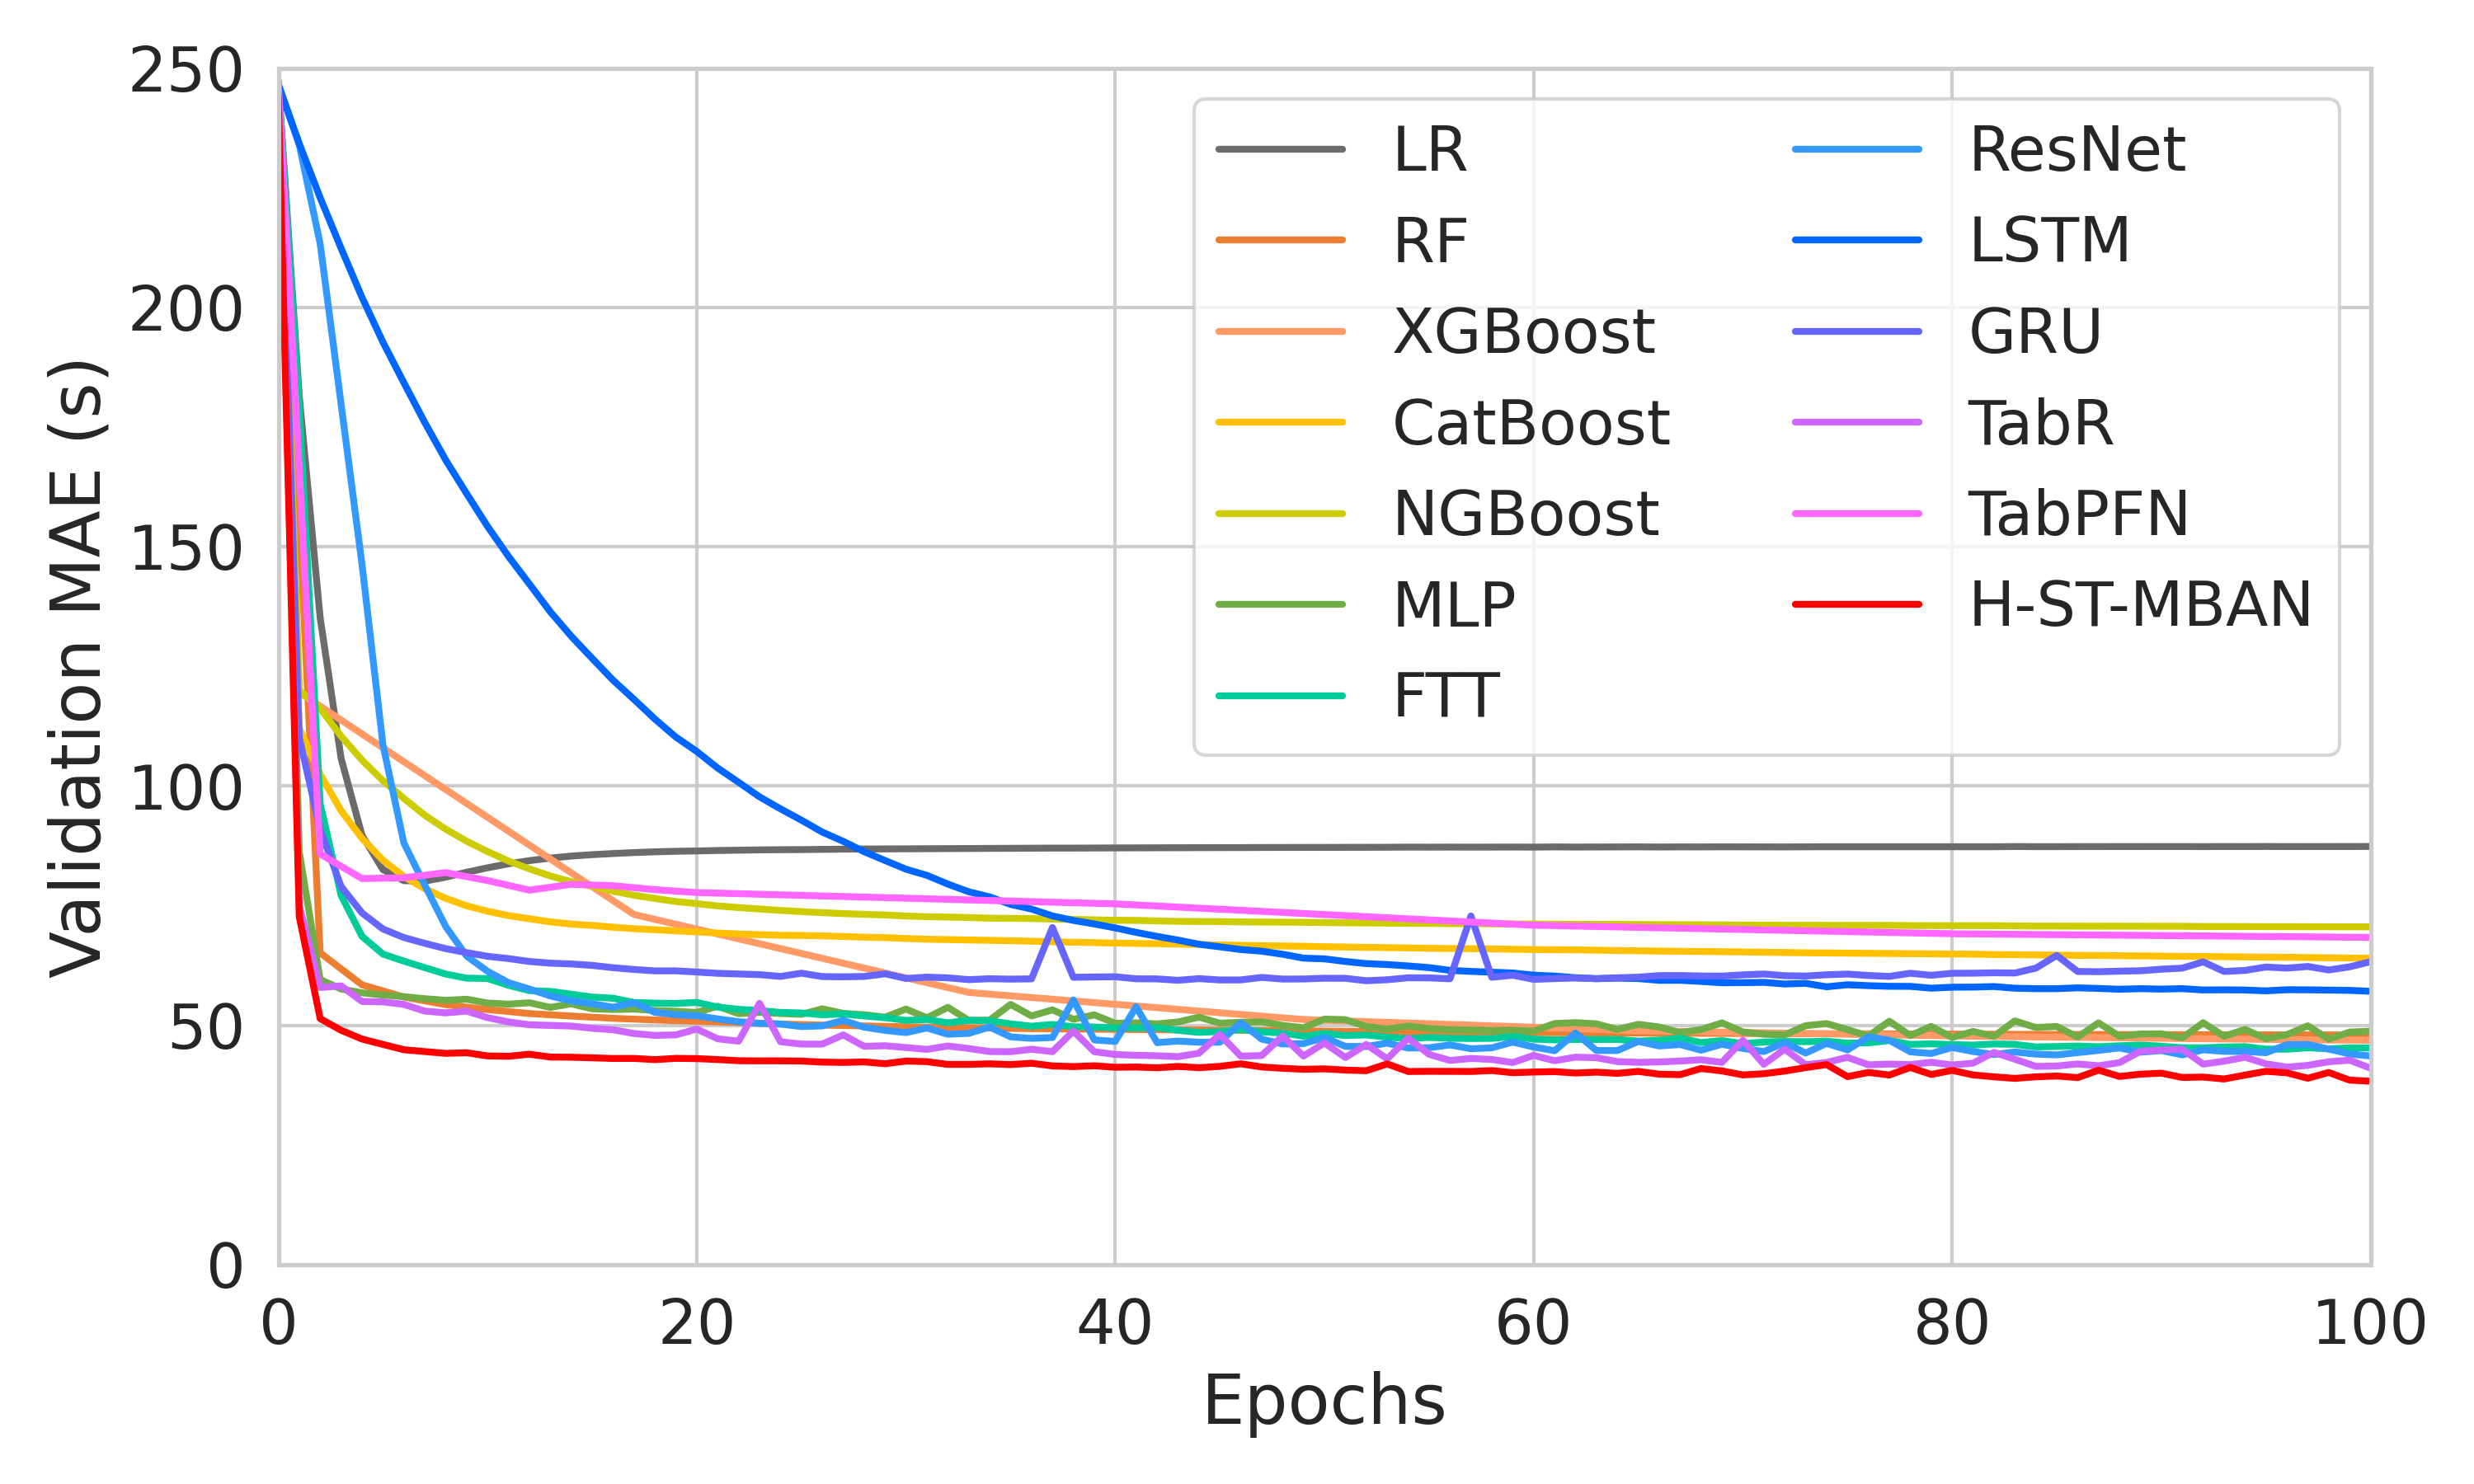
\includegraphics[width=\columnwidth]{figure/G1_learning_curves_All.png}
\caption{G1 (Learning Curves): Convergence of H-ST-MBAN compared to baseline models. ML model iterations are aligned with DL epochs for a fair comparison.}
\label{fig:G1}
\end{figure}

\subsection{G2: Ablation Study}
To evaluate the contribution of the proposed architecture, we conducted an ablation study by modifying the H-ST-MBAN components.
As illustrated in Figure~\ref{fig:G2}, we evaluate three degraded variants: 1) \textit{w/o Attn}, which replaces the multi-head self-attention mechanism with simple concatenation; 2) \textit{w/o XGB}, which relies solely on the neural network stream by omitting the GBDT prior; and 3) \textit{Early Fusion}, which concatenates features before encoding instead of using the independent branch structure. This component breakdown isolates the individual contribution of each architectural feature. The results show that the \textit{w/o XGB} variant experiences an increase in prediction error, confirming the necessity of integrating the tabular prior to handle decision boundaries that the neural network struggles to learn alone. The \textit{Early Fusion} variant also exhibits higher error, indicating that the heterogeneous nature of vehicular data benefits from semantic branching to prevent gradient conflicts during encoding. Finally, removing the attention layer in \textit{w/o Attn} degrades convergence and increases error, showing that multi-head self-attention routes the relevant bottleneck features depending on the specific intersection context. The full H-ST-MBAN model achieves the lowest error and fastest convergence. This collective behavior confirms the complementary relationship between gradient-boosted tabular priors and neural representation learning, where the GBDT stream establishes baseline decisions and the multi-branch neural network stream refines spatio-temporal details.

\begin{figure}[!t]
\centering
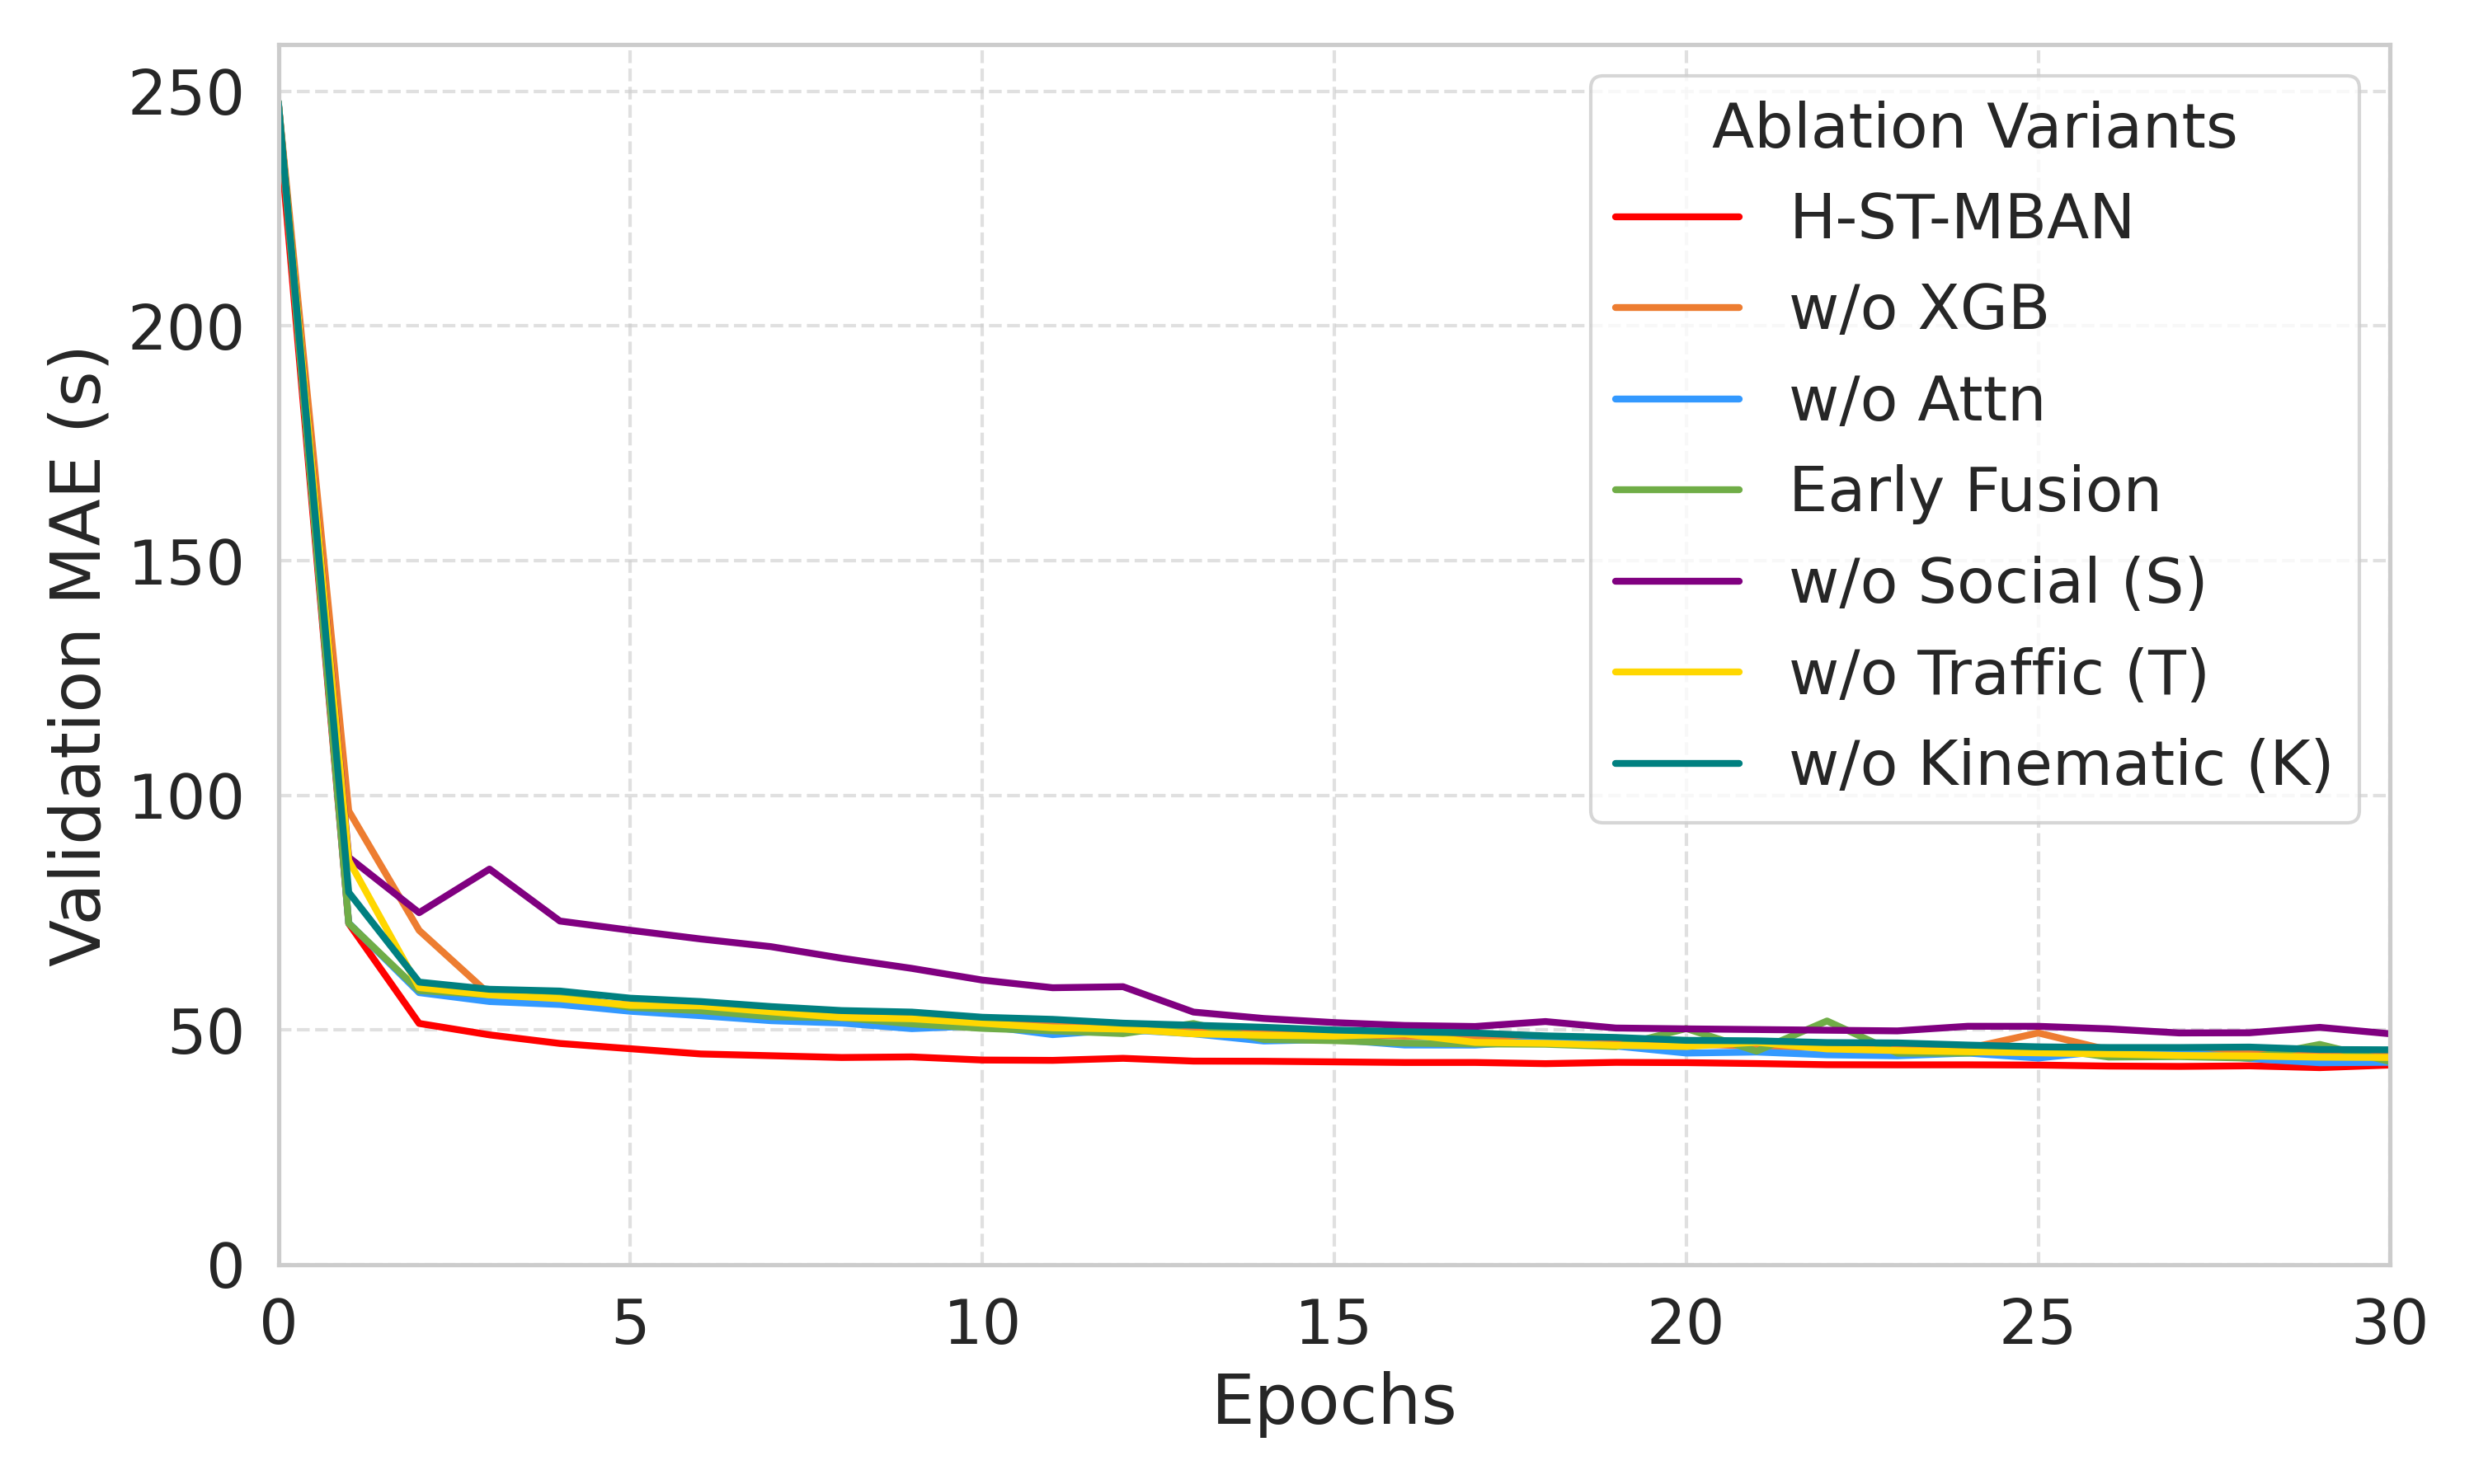
\includegraphics[width=\columnwidth]{figure/G2_ablation_study.png}
\caption{G2 (Ablation Study): Performance of H-ST-MBAN compared to w/o Attn, w/o XGB, and Early Fusion variants.}
\label{fig:G2}
\end{figure}

\subsection{G3: Prediction Accuracy}
Table~\ref{tab:accuracy} summarizes the global prediction performance.
H-ST-MBAN yields an MAE of 44.32~s, improving upon the second-best baseline, ResNet, which yields an MAE of 47.10~s. Traditional sequential models, namely LSTM and GRU, show higher error, exhibiting higher MAEs of 96.90~s and 101.75~s, respectively, which may be attributed to the difficulty of inferring temporal dynamics from a single event-driven snapshot.
The reduction in MAE achieved by H-ST-MBAN compared to ResNet is primarily due to the incorporation of the gradient boosting tabular prior stream, which models sharp decision boundaries.
In contrast, pure deep neural network structures struggle to learn these non-linear tabular divisions from unstructured variables.
Additionally, the multi-branch self-attention fusion allows H-ST-MBAN to weight dynamic spatial and temporal components based on signal timings, which mitigates regression error.

Figure~\ref{fig:G3} visualizes the True vs. Predicted dwell times for both current and next targets.
In these plots, H-ST-MBAN demonstrates tighter clustering along the identity line, indicating stability against outliers that typically disrupt V2I schedules.
The prediction for the next RSU dwell time, denoted as $\hat{\tau}_\text{nxt}$, shows slightly more variance and error than the current RSU dwell time, $\hat{\tau}_\text{cur}$. This variance is physically intuitive because downstream traffic conditions at the next intersection are subject to additional random perturbations during the inter-RSU traversal interval. Despite this inherent uncertainty, the proposed design maintains a tight error boundary, confirming the benefit of incorporating multi-intersection social features.
This occurs because predicting further into the future involves a more complex spatial-temporal space, particularly since the vehicle can branch into one of four possible next RSUs at the upcoming intersection.
To address this spatial-temporal uncertainty, the caching scheduler can implement a dynamic correction factor that adjusts prefetching thresholds based on branching probabilities.
This compensation mechanism mitigates the impact of estimation variance on subsequent roadside edge cache hit rates.

\begin{table*}[!t]
\centering
\caption{Global Prediction Accuracy Across 13 Models. H-ST-MBAN achieves the lowest MAE and RMSE.}
\label{tab:accuracy}
\begin{tabular}{lcccc}
\toprule
\textbf{Model} & \textbf{MAE (s) $\downarrow$} & \textbf{RMSE (s) $\downarrow$} & \textbf{MAPE (\%) $\downarrow$} & \textbf{$R^2$ $\uparrow$} \\
\midrule
\textbf{H-ST-MBAN} & \textbf{44.32} & \textbf{90.54} & \textbf{17.90} & \textbf{0.8618} \\
ResNet & 47.10 & 92.27 & 23.16 & 0.8565 \\
TabPFN & 66.62 & 152.33 & 21.30 & 0.6089 \\
TabR & 80.59 & 170.40 & 27.32 & 0.5106 \\
XGB & 81.95 & 181.94 & 23.88 & 0.4420 \\
CatBoost & 83.02 & 187.83 & 24.72 & 0.4053 \\
RF & 83.75 & 185.30 & 26.59 & 0.4212 \\
LSTM & 96.90 & 196.65 & 32.44 & 0.3481 \\
LR & 97.42 & 199.67 & 49.57 & 0.3280 \\
GRU & 101.75 & 201.36 & 40.40 & 0.3165 \\
FTT & 103.52 & 194.94 & 39.61 & 0.3594 \\
MLP & 108.02 & 212.61 & 35.89 & 0.2380 \\
NGBoost & 109.18 & 199.09 & 76.12 & 0.3318 \\
\bottomrule
\end{tabular}
\end{table*}

\begin{figure}[!t]
\centering
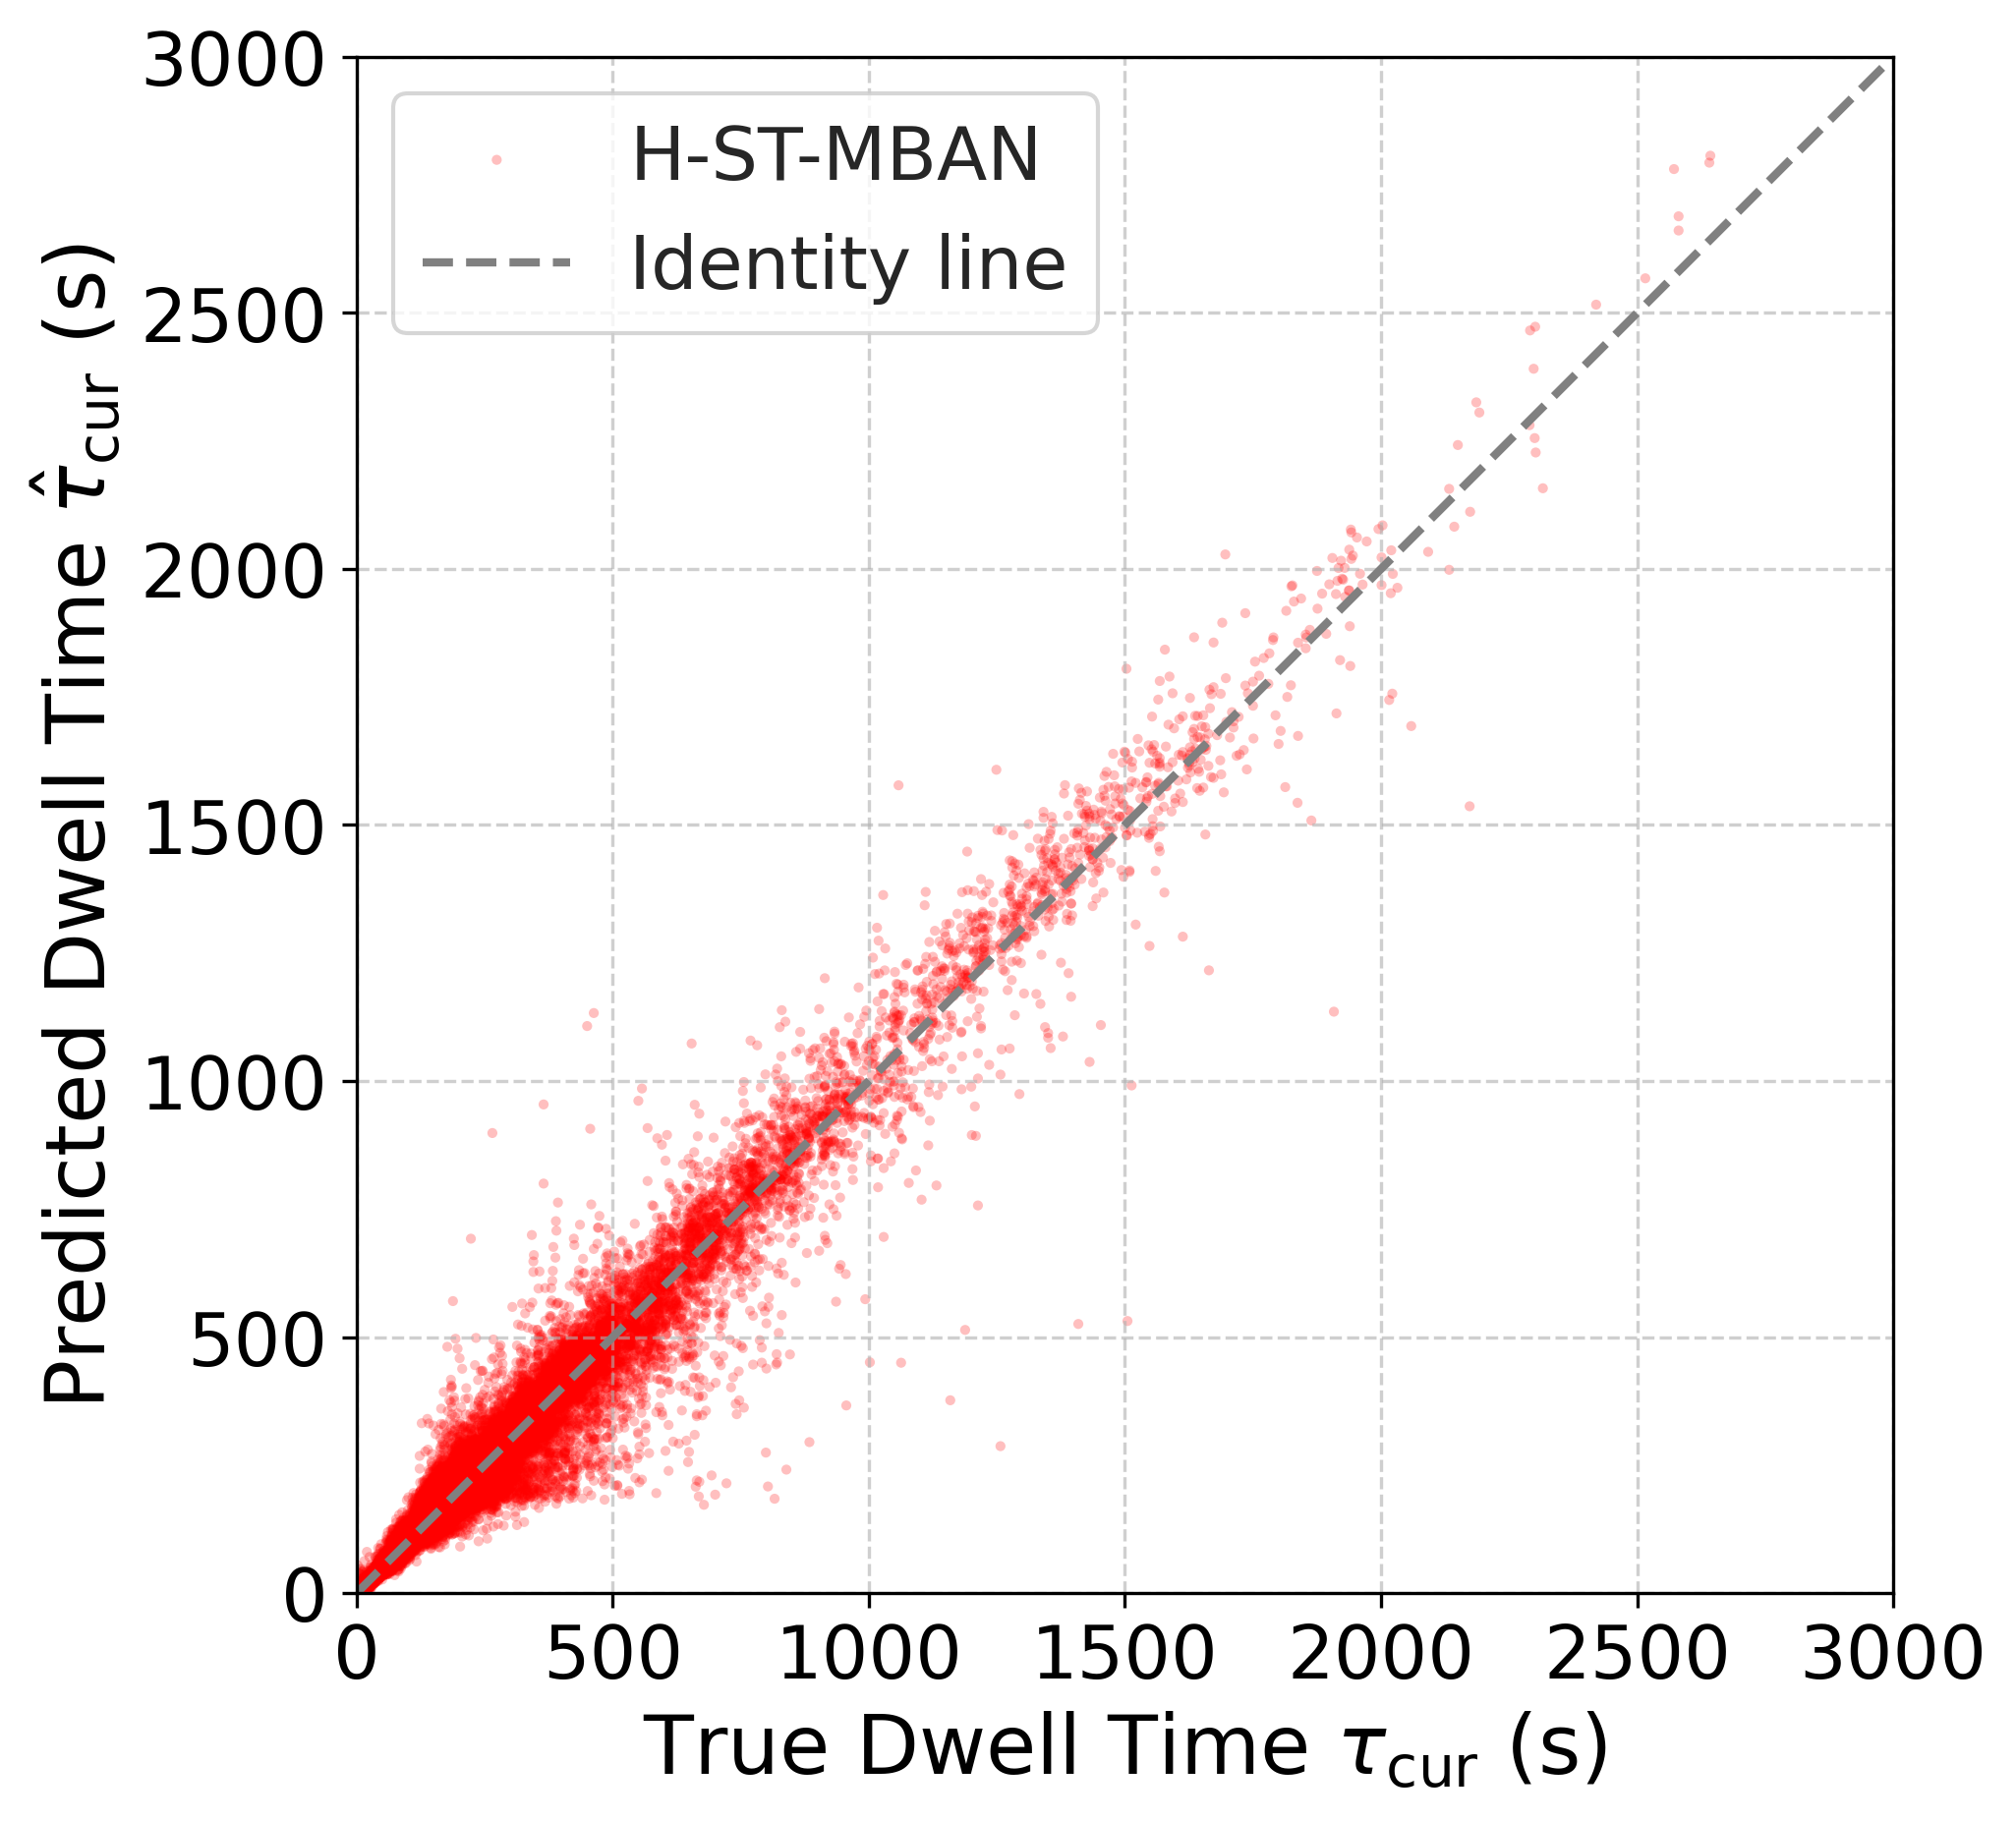
\includegraphics[width=0.48\columnwidth]{figure/G3-1_pred_vs_true_cur.png}
\hfill
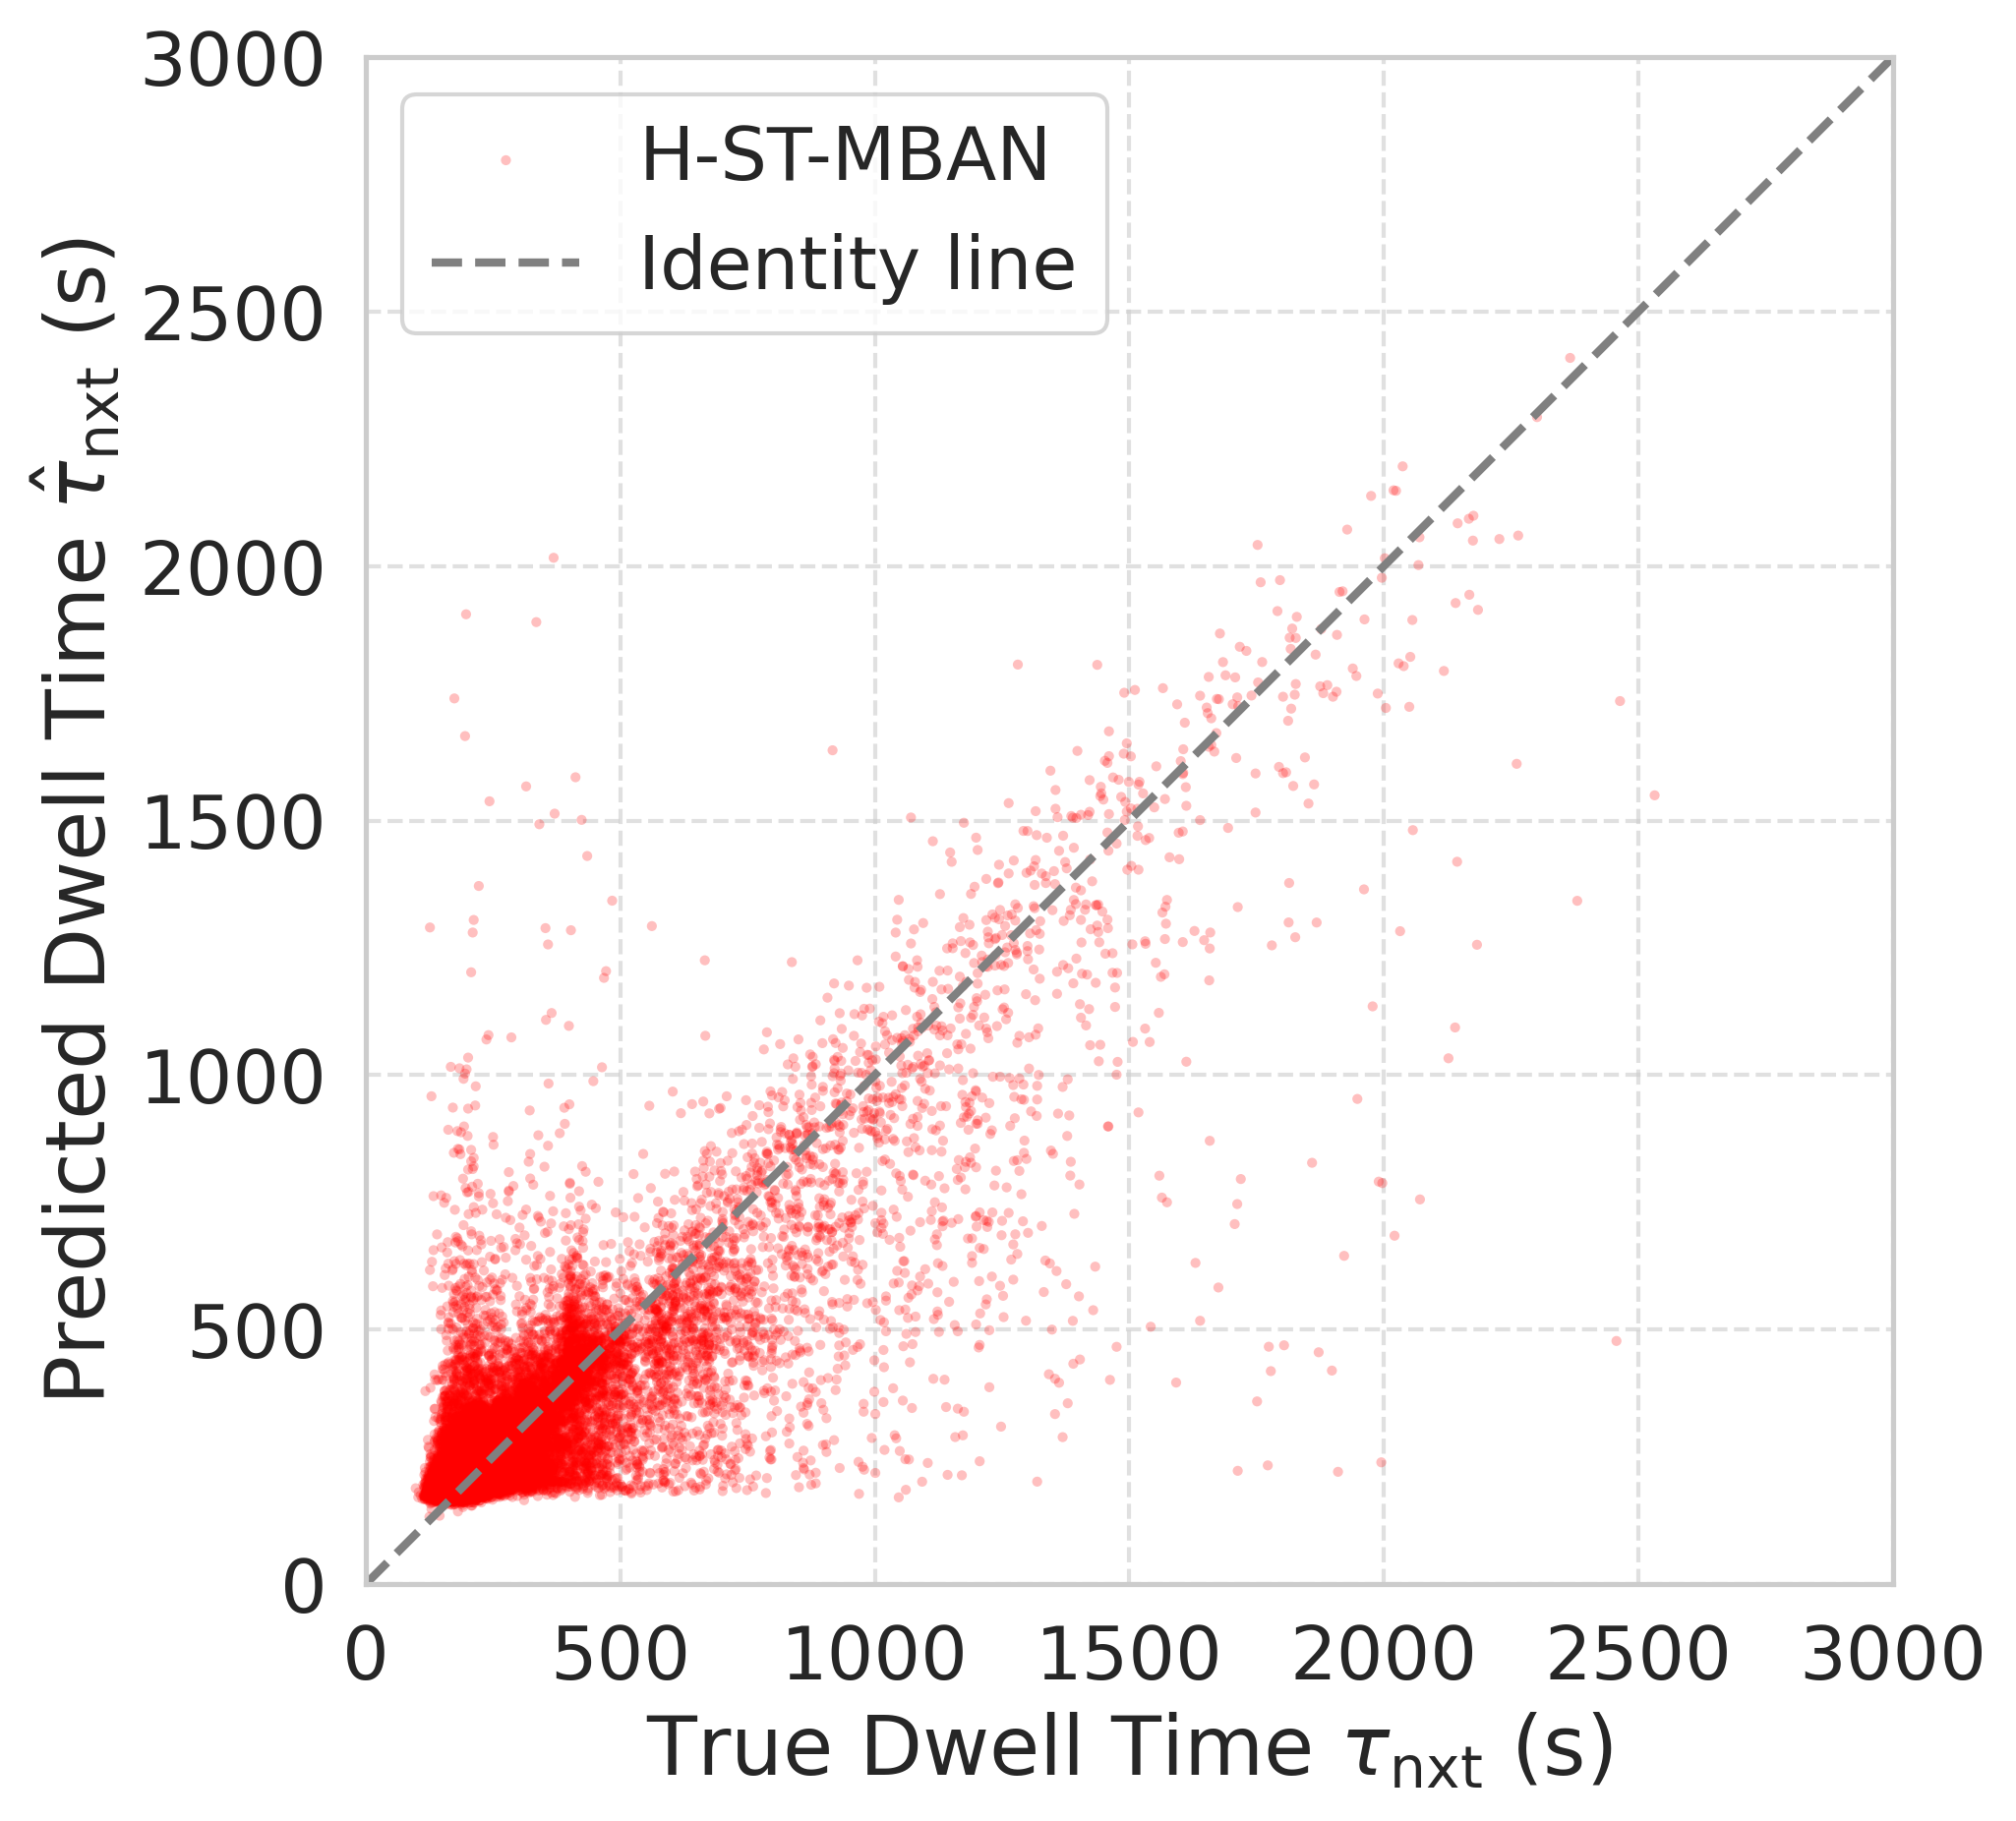
\includegraphics[width=0.48\columnwidth]{figure/G3-2_pred_vs_true_nxt.png}
\caption{G3 (Prediction Accuracy): Scatter plots of True vs. Predicted Dwell Time for current target, $\hat{\tau}_\text{cur}$, on the left and next target, $\hat{\tau}_\text{nxt}$, on the right.}
\label{fig:G3}
\end{figure}

\subsection{G4: Optimal Queue Size Analysis}
The global pre-training phase is executed on a high-performance workstation equipped with an Intel Core i9-10900X CPU, 128 GB of RAM, and four NVIDIA GeForce RTX 3090 GPUs, while the local fine-tuning phase must be viable on resource-constrained RSU edge hardware.
To evaluate edge feasibility, we analyze the computational complexity of the model and its memory footprint.
In dynamic vehicular environments, edge computing boards operate under strict thermal and electrical constraints, which limits the deployment of oversized deep learning parameters.
Moreover, because dwell-time prediction must be completed within milliseconds of a request packet arrival, memory access latency must be minimized to avoid buffering bottlenecks.
These edge constraints necessitate lightweight models that do not exceed local computing bounds while maintaining accuracy.
Specifically, empirical measurements during the first round of local fine-tuning demonstrate a total training time of 1.93 seconds and a peak memory consumption of 47.69 MB.
This lightweight resource requirement fits within the thermal and electrical limits of typical RSU hardware units.
Thus, real-time localized adaptation is computationally feasible under dynamic vehicular edge environments.

As shown in Figure~\ref{fig:G4-1} and Figure~\ref{fig:G4-2}, we analyze the trade-off between the fine-tuning queue size and local prediction stability. A queue size of 5000 is chosen as the optimal operating parameter based on three analytical justifications. First, this value represents the knee of the curve regarding cost-effectiveness, where the marginal gain in stability, which represents a variance reduction, drops when scaling past 5000. Second, to ensure statistical confidence, the MAE standard deviation, represented by SEM, is below 1.0, yielding approximately 0.29~s, at $Q=5000$, preventing erratic model updates. Third, this configuration provides an adequate ITS SLA margin. According to ITS recommended standards, caching and model updates should occur every 15--60 minutes \cite{31}. Accumulating a queue of 5000 snapshots takes approximately 43 minutes, placing the update frequency in the middle of this 15--60 minutes ITS standard interval and providing a safety buffer against varying traffic density.

\begin{figure}[!t]
\centering
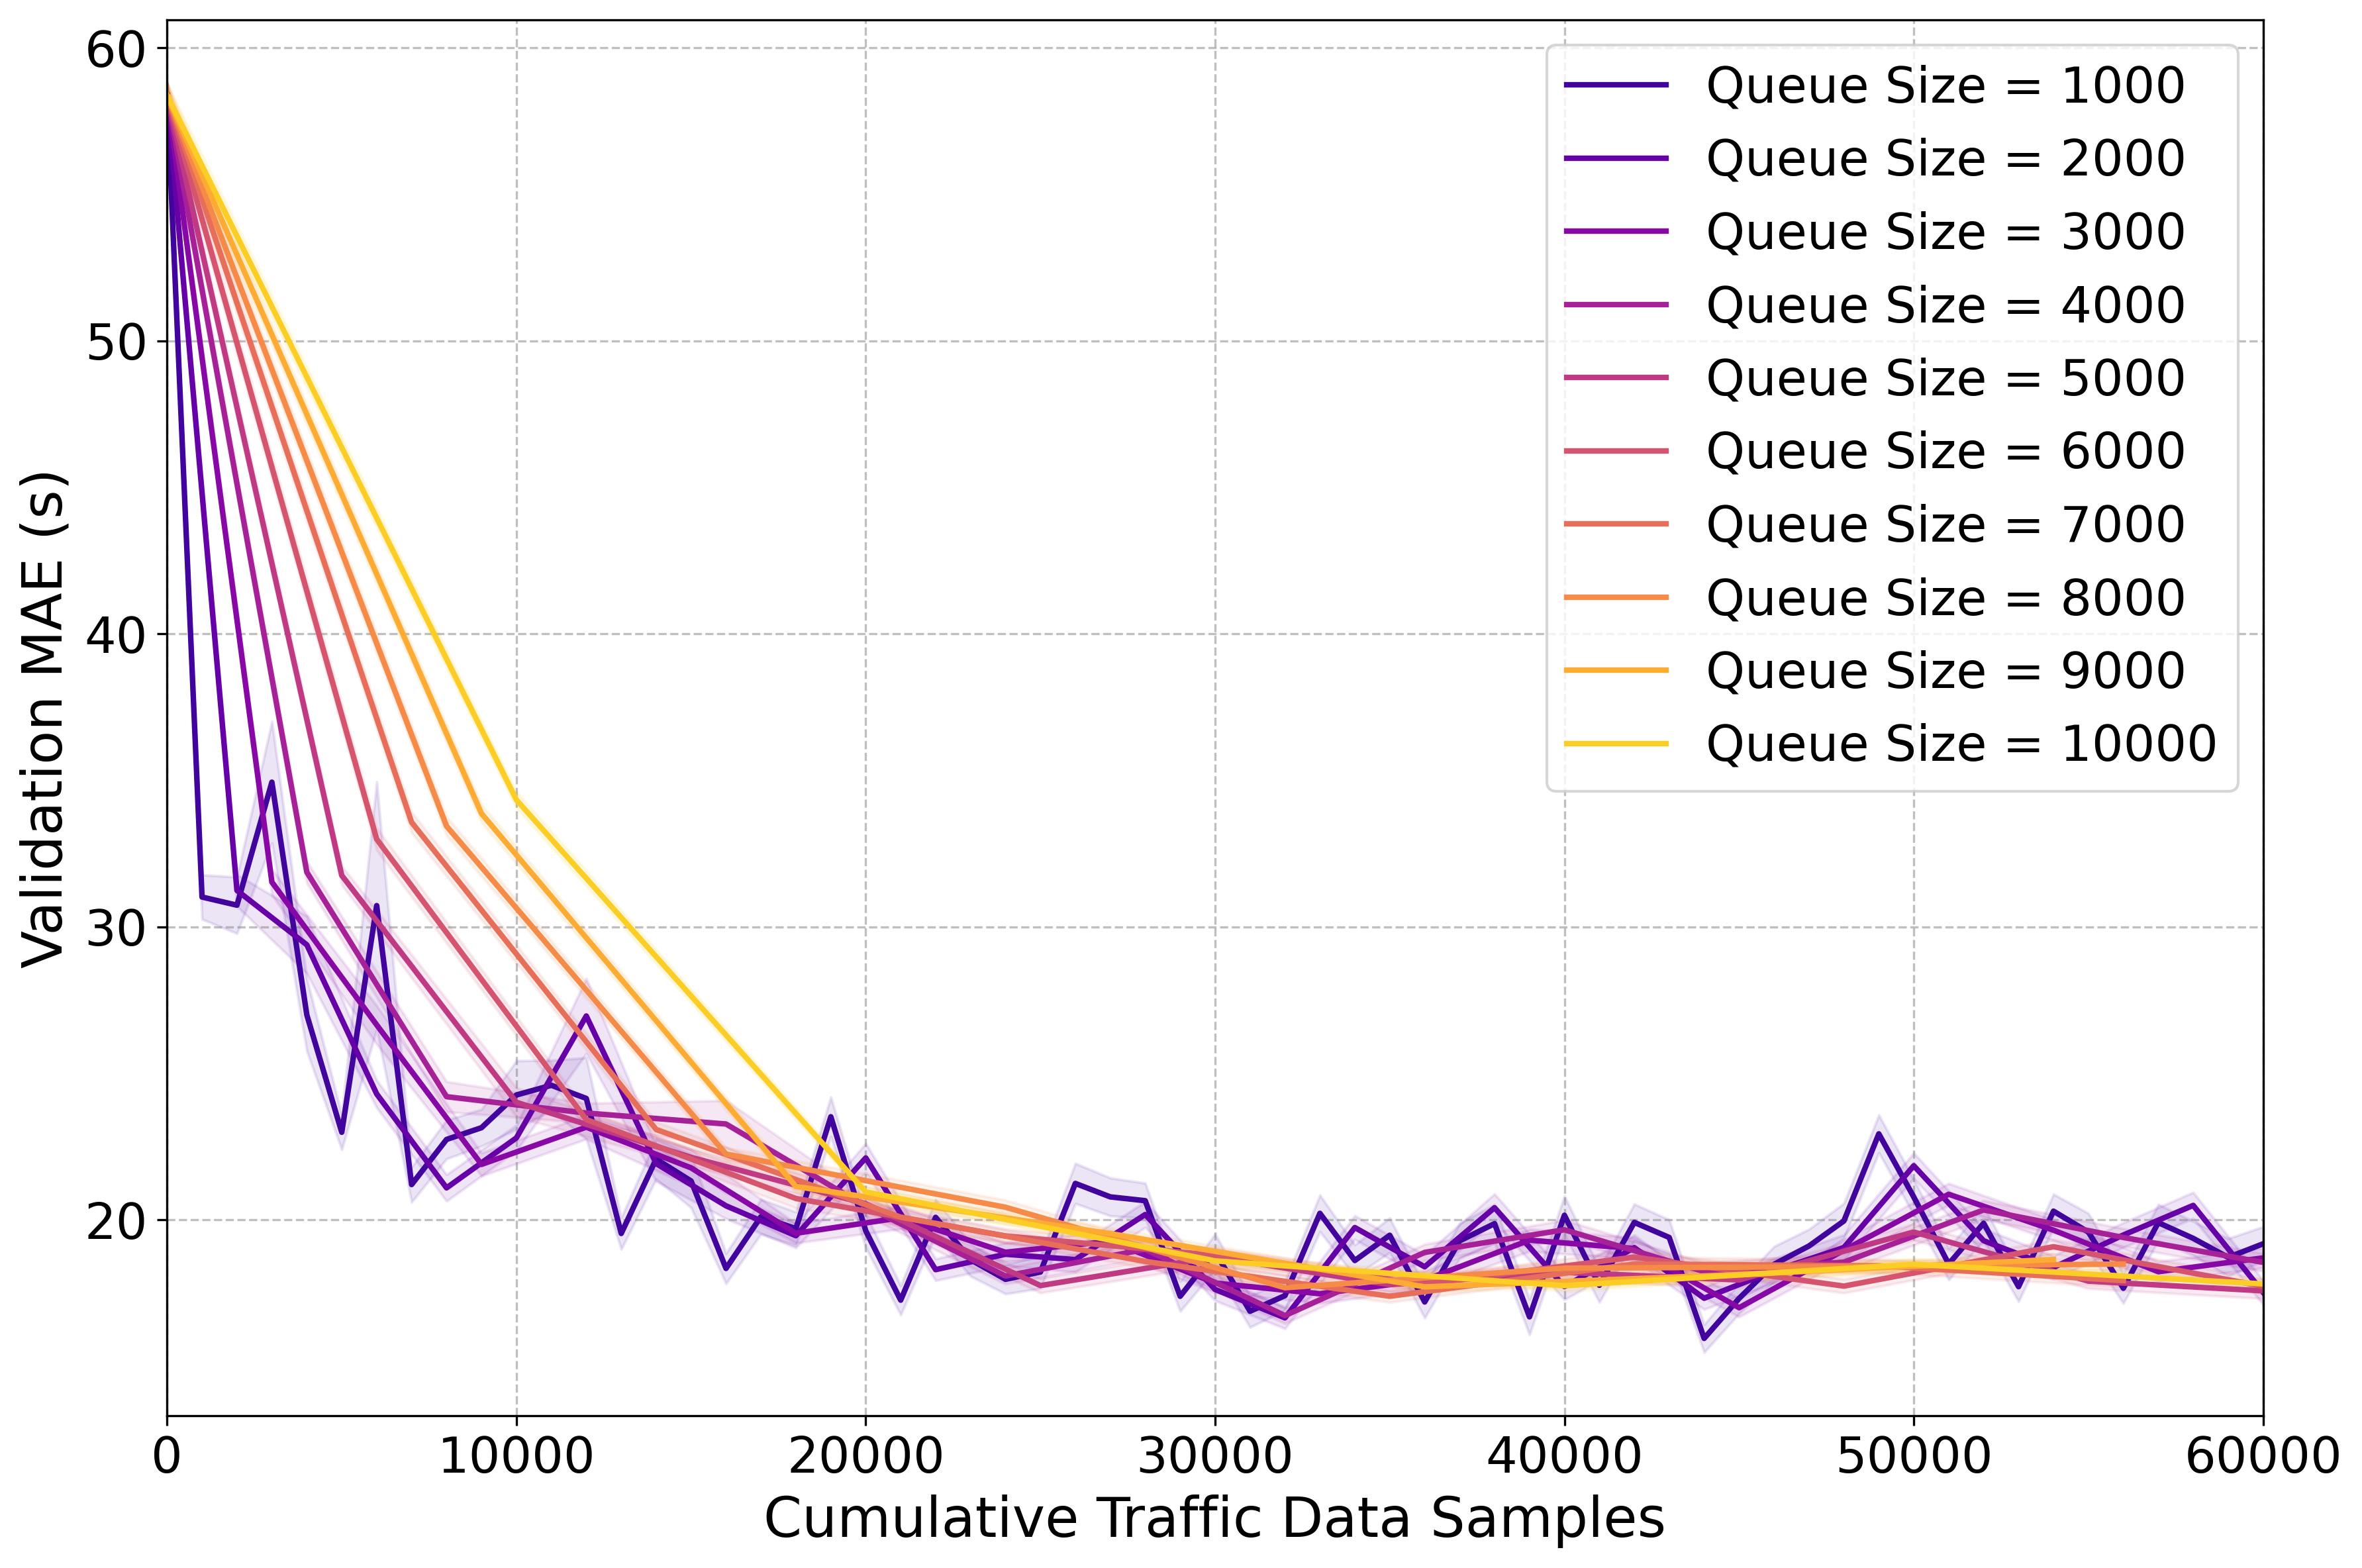
\includegraphics[width=\columnwidth]{figure/G4-1_cumulative_mae_validation.png}
\caption{H-ST-MBAN cumulative validation MAE curves by queue size.}
\label{fig:G4-1}
\end{figure}

\begin{figure}[!t]
\centering
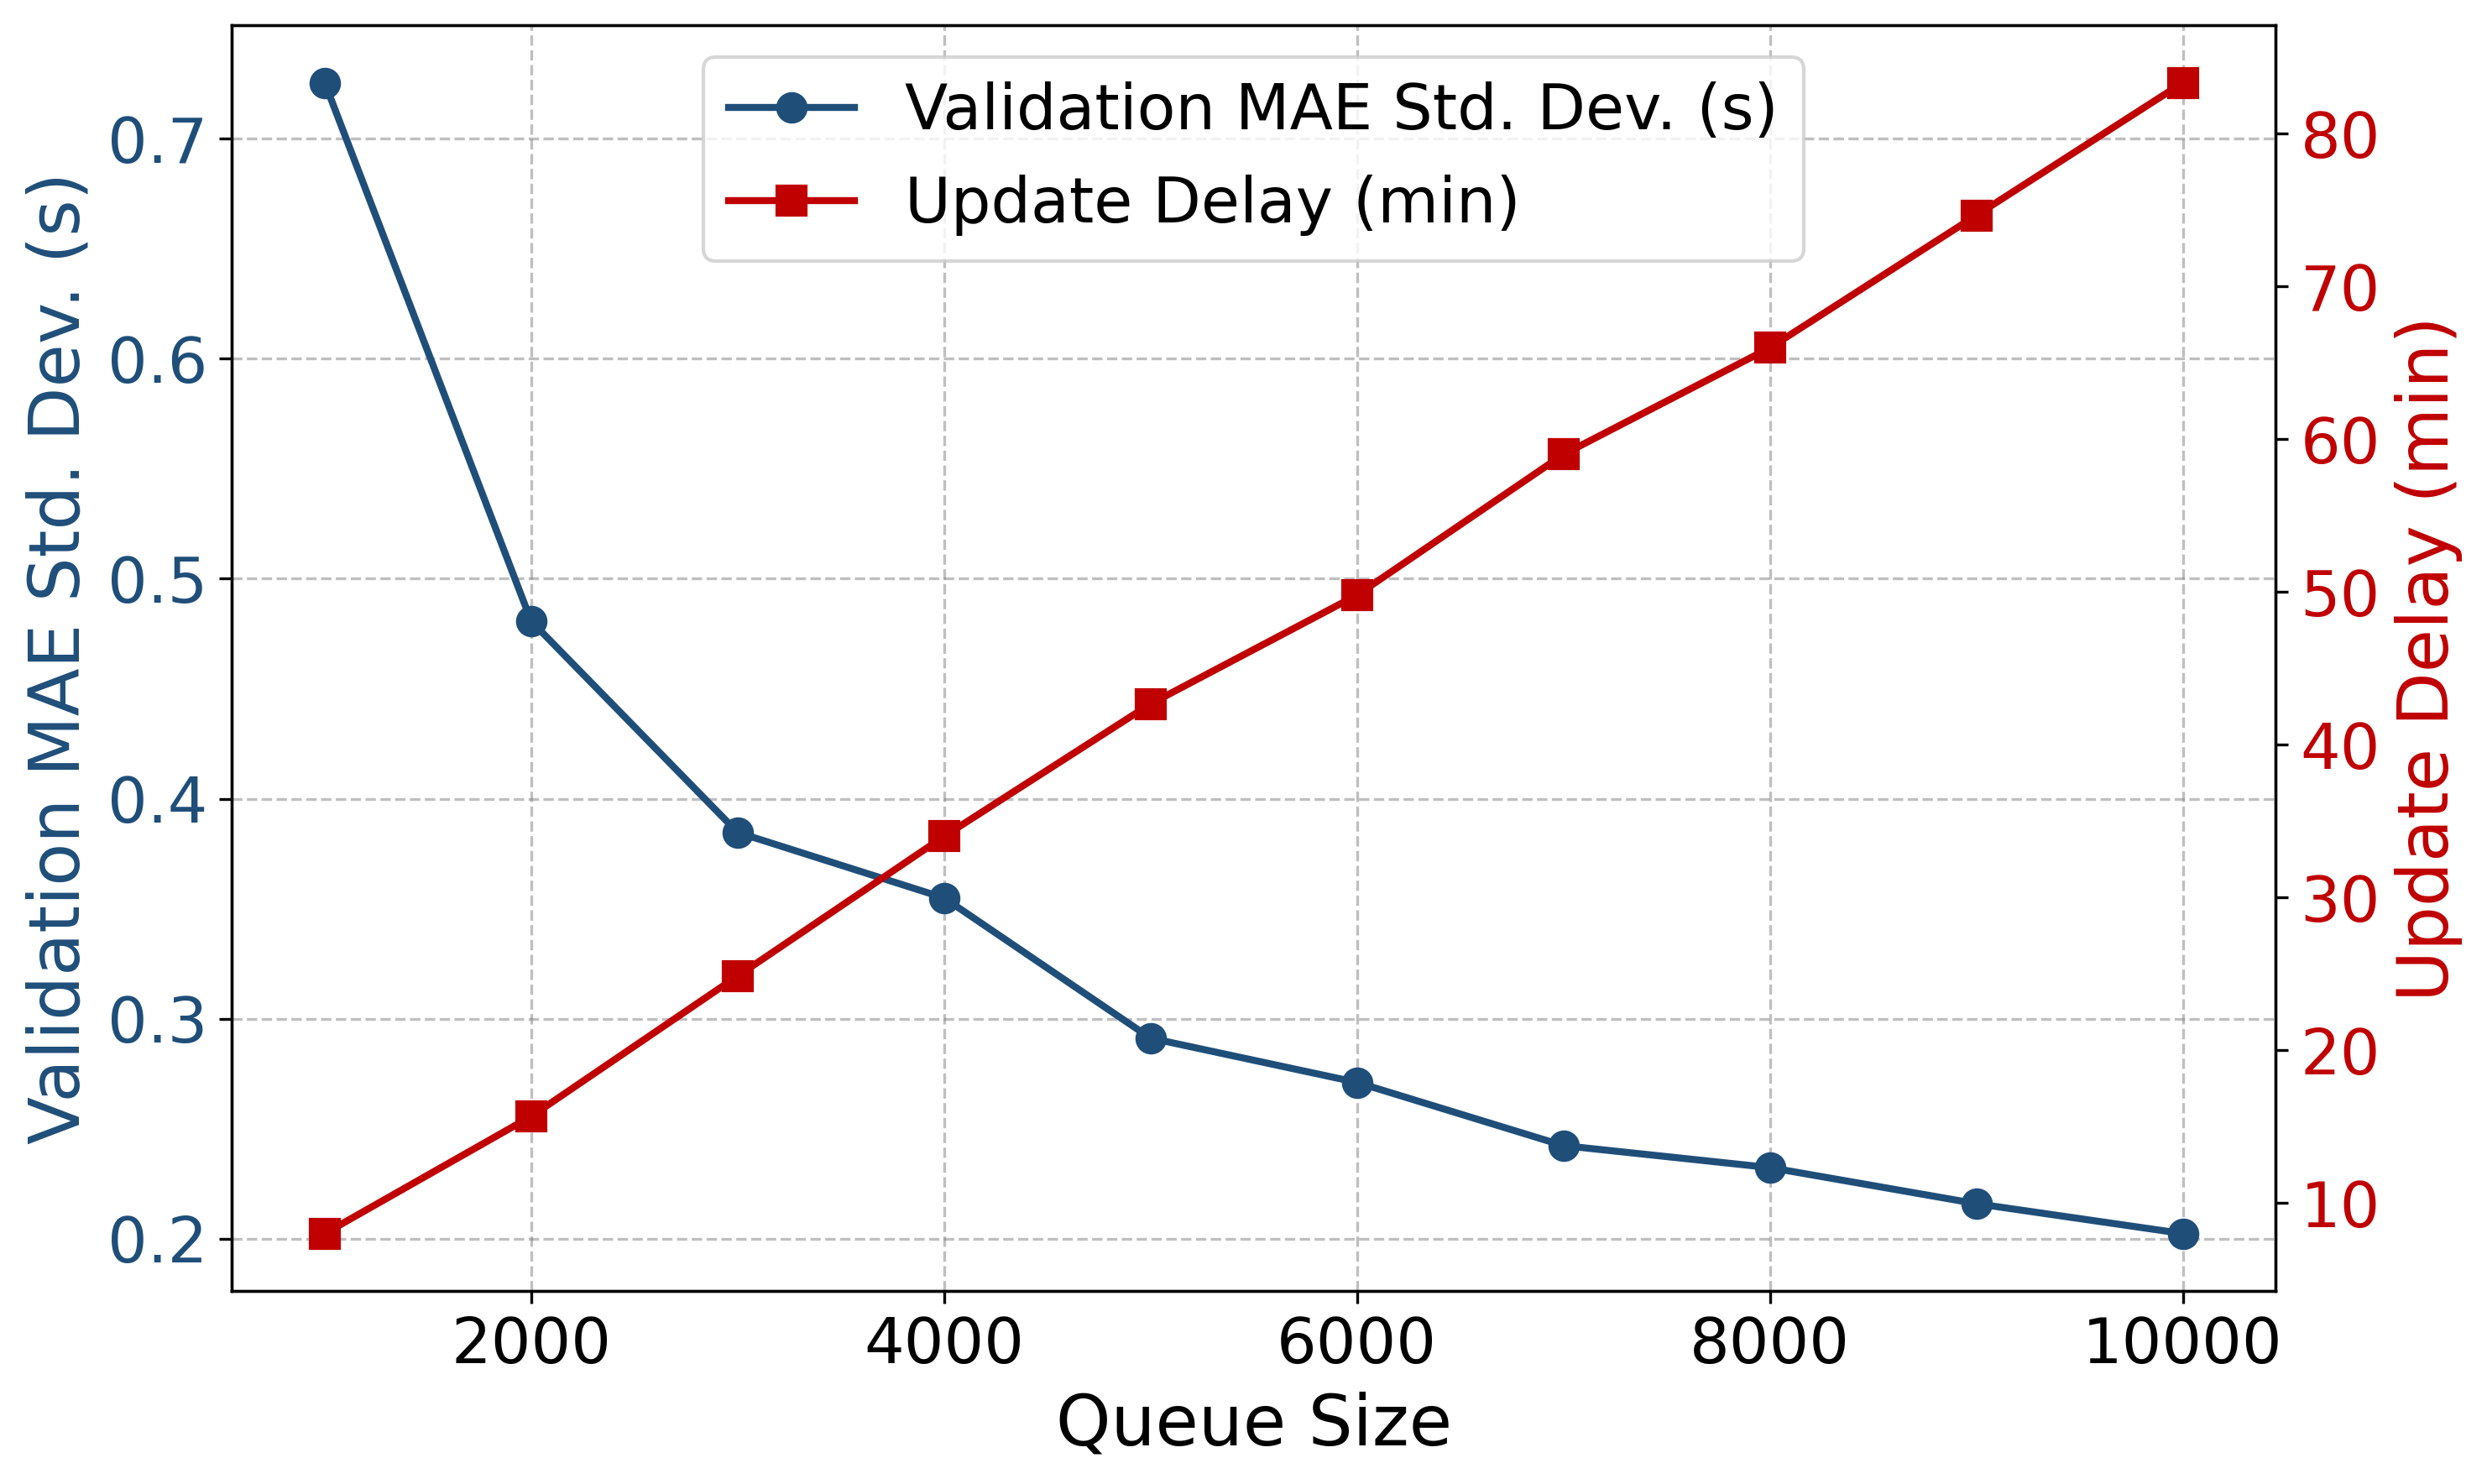
\includegraphics[width=\columnwidth]{figure/G4-2_queue_size_analysis.png}
\caption{Impact of queue size on MAE Std. Dev. (SEM) and Update Delay.}
\label{fig:G4-2}
\end{figure}

\begin{table}[!t]
\centering
\caption{Fine-Tuning Complexity and RSU Edge Feasibility (1 Round, Q=5000)}
\label{tab:complexity}
\begin{tabular}{@{}lc@{}}
\toprule
\textbf{Metric} & \textbf{H-ST-MBAN} \\
\midrule
Parameters (M) & 1.385 \\
Model Size (MB) & 5.32 \\
Training Time (s) & 1.93 \\
Peak Memory (MB) & 47.69 \\
FLOPs (M) & 198,750 \\
\bottomrule
\end{tabular}
\end{table}

\subsection{G5: Online Fine-Tuning Performance}
Figure~\ref{fig:G5} and Table~\ref{tab:finetune_accuracy} present the online fine-tuning performance. As quantitatively summarized in Table~\ref{tab:finetune_accuracy}, H-ST-MBAN achieves the lowest average MAE of 20.33~\text{s}, outperforming all baseline models including the FTT model, which records 40.62~\text{s}. In addition, the MAE progression in Figure~\ref{fig:G5} visually demonstrates H-ST-MBAN's performance over the ML/NN baselines by preventing catastrophic forgetting. The proposed dual-model fine-tuning mechanism updates the local weights, maintaining a low error rate across continuous operation. In contrast, baseline models that lack this localized adaptation experience higher error over time as they fail to adapt to evolving traffic patterns. This performance advantage highlights the robustness of combining GBDT-based boundary partition with deep temporal feature learning during online adaptation.

Specifically, Table~\ref{tab:finetune_accuracy} shows that H-ST-MBAN reduces its prediction error from a Global MAE of 58.39~s to a Final MAE of 17.58~s after fine-tuning. This improvement is accompanied by a low standard deviation of 4.12~s, indicating that the local adaptation process is highly stable. In contrast, standard deep learning baselines such as MLP, ResNet, and TabR exhibit an increase in error during the local fine-tuning phase. Due to local overfitting and gradient instability under resource-constrained conditions, their Average MAEs increase to over 100~s, reaching 100.91~s, 103.58~s, and 106.38~s for MLP, ResNet, and TabR, respectively. Similarly, their standard deviations exceed 20~s, yielding 21.04~s, 23.86~s, and 26.74~s. This numerical contrast reveals that these baseline architectures suffer from weight spiking and unstable optimization trajectories when updated with local edge queues. As a result, H-ST-MBAN maintains predictive reliability under dynamic traffic environments, whereas conventional neural network models fail to adapt. Meanwhile, traditional sequential baselines such as LSTM maintain a relatively stable error, yielding an Average MAE of 52.06~s, yet fail to approach the performance of H-ST-MBAN.

During the online adaptation process, the RSU edge node periodically accumulates vehicular state variables $X_v$ from incoming V2I content request packets into a local storage buffer. Under dynamic traffic environments, the inflow of outlier samples during this online training phase can induce gradient instability, which degrades deep learning weight configuration. H-ST-MBAN addresses this vulnerability by incorporating a steady-state filtering pre-processor at the RSU, which screens incoming state variables prior to gradient calculation. Compared to tree ensembles such as XGBoost that rely on fixed global weights and lack online model updates, H-ST-MBAN dynamically adjusts local weights using the local snapshot queue. Once the fine-tuning process completes, the updated model weights are applied to estimate the dwell duration, and the resulting prediction is transmitted to the caching scheduler to determine the prefetching queue configuration. This real-time sanitization phase prevents noisy updates, thereby preserving the structural stability of the globally trained prior weights.

During the online fine-tuning process at the RSU edge node, standard deep learning baselines frequently exhibit performance degradation and sudden weight spikes in their loss curves. This instability during local adaptation originates from four primary structural causes under the dynamic vehicular network environment. First, local overfitting occurs due to data sparsity within the constrained local snapshot queue of size $Q=5000$, which fails to represent the broader traffic distribution. Second, standard neural networks experience catastrophic forgetting of globally acquired representations because they lack explicit regularization constraints to preserve pre-trained knowledge during local gradient steps. Third, unexpected traffic anomalies introduce outlier samples, such as vehicles with dwell times exceeding 300 seconds, which leads to gradient pollution during backpropagation. Fourth, updating the entire parameter set through full fine-tuning under highly non-stationary edge traffic dynamics causes the optimization trajectory to diverge.

To overcome these vulnerabilities and stabilize the parameter update path, four corresponding mitigation strategies are required, which are structurally addressed by the H-ST-MBAN architecture. First, parameter-efficient fine-tuning or localized training of gating layers minimizes parameter drift, a mechanism realized by the gating fusion structure in H-ST-MBAN to control neural network weight variations. Second, global weight anchoring restricts the deviation between the local parameters and the globally pre-trained model weights. Third, applying a cosine annealing learning rate scheduler and enhanced weight decay prevents abrupt weight updates under noisy inputs. Fourth, the RSU utilizes a steady-state filtering pre-processor to sanitize the local queue before initiating gradient calculations. Once the fine-tuning iteration completes, the RSU computes the estimated vehicle dwell duration and transmits this value to the prefetching scheduler to configure the edge cache.

\begin{figure*}[!t]
\centering
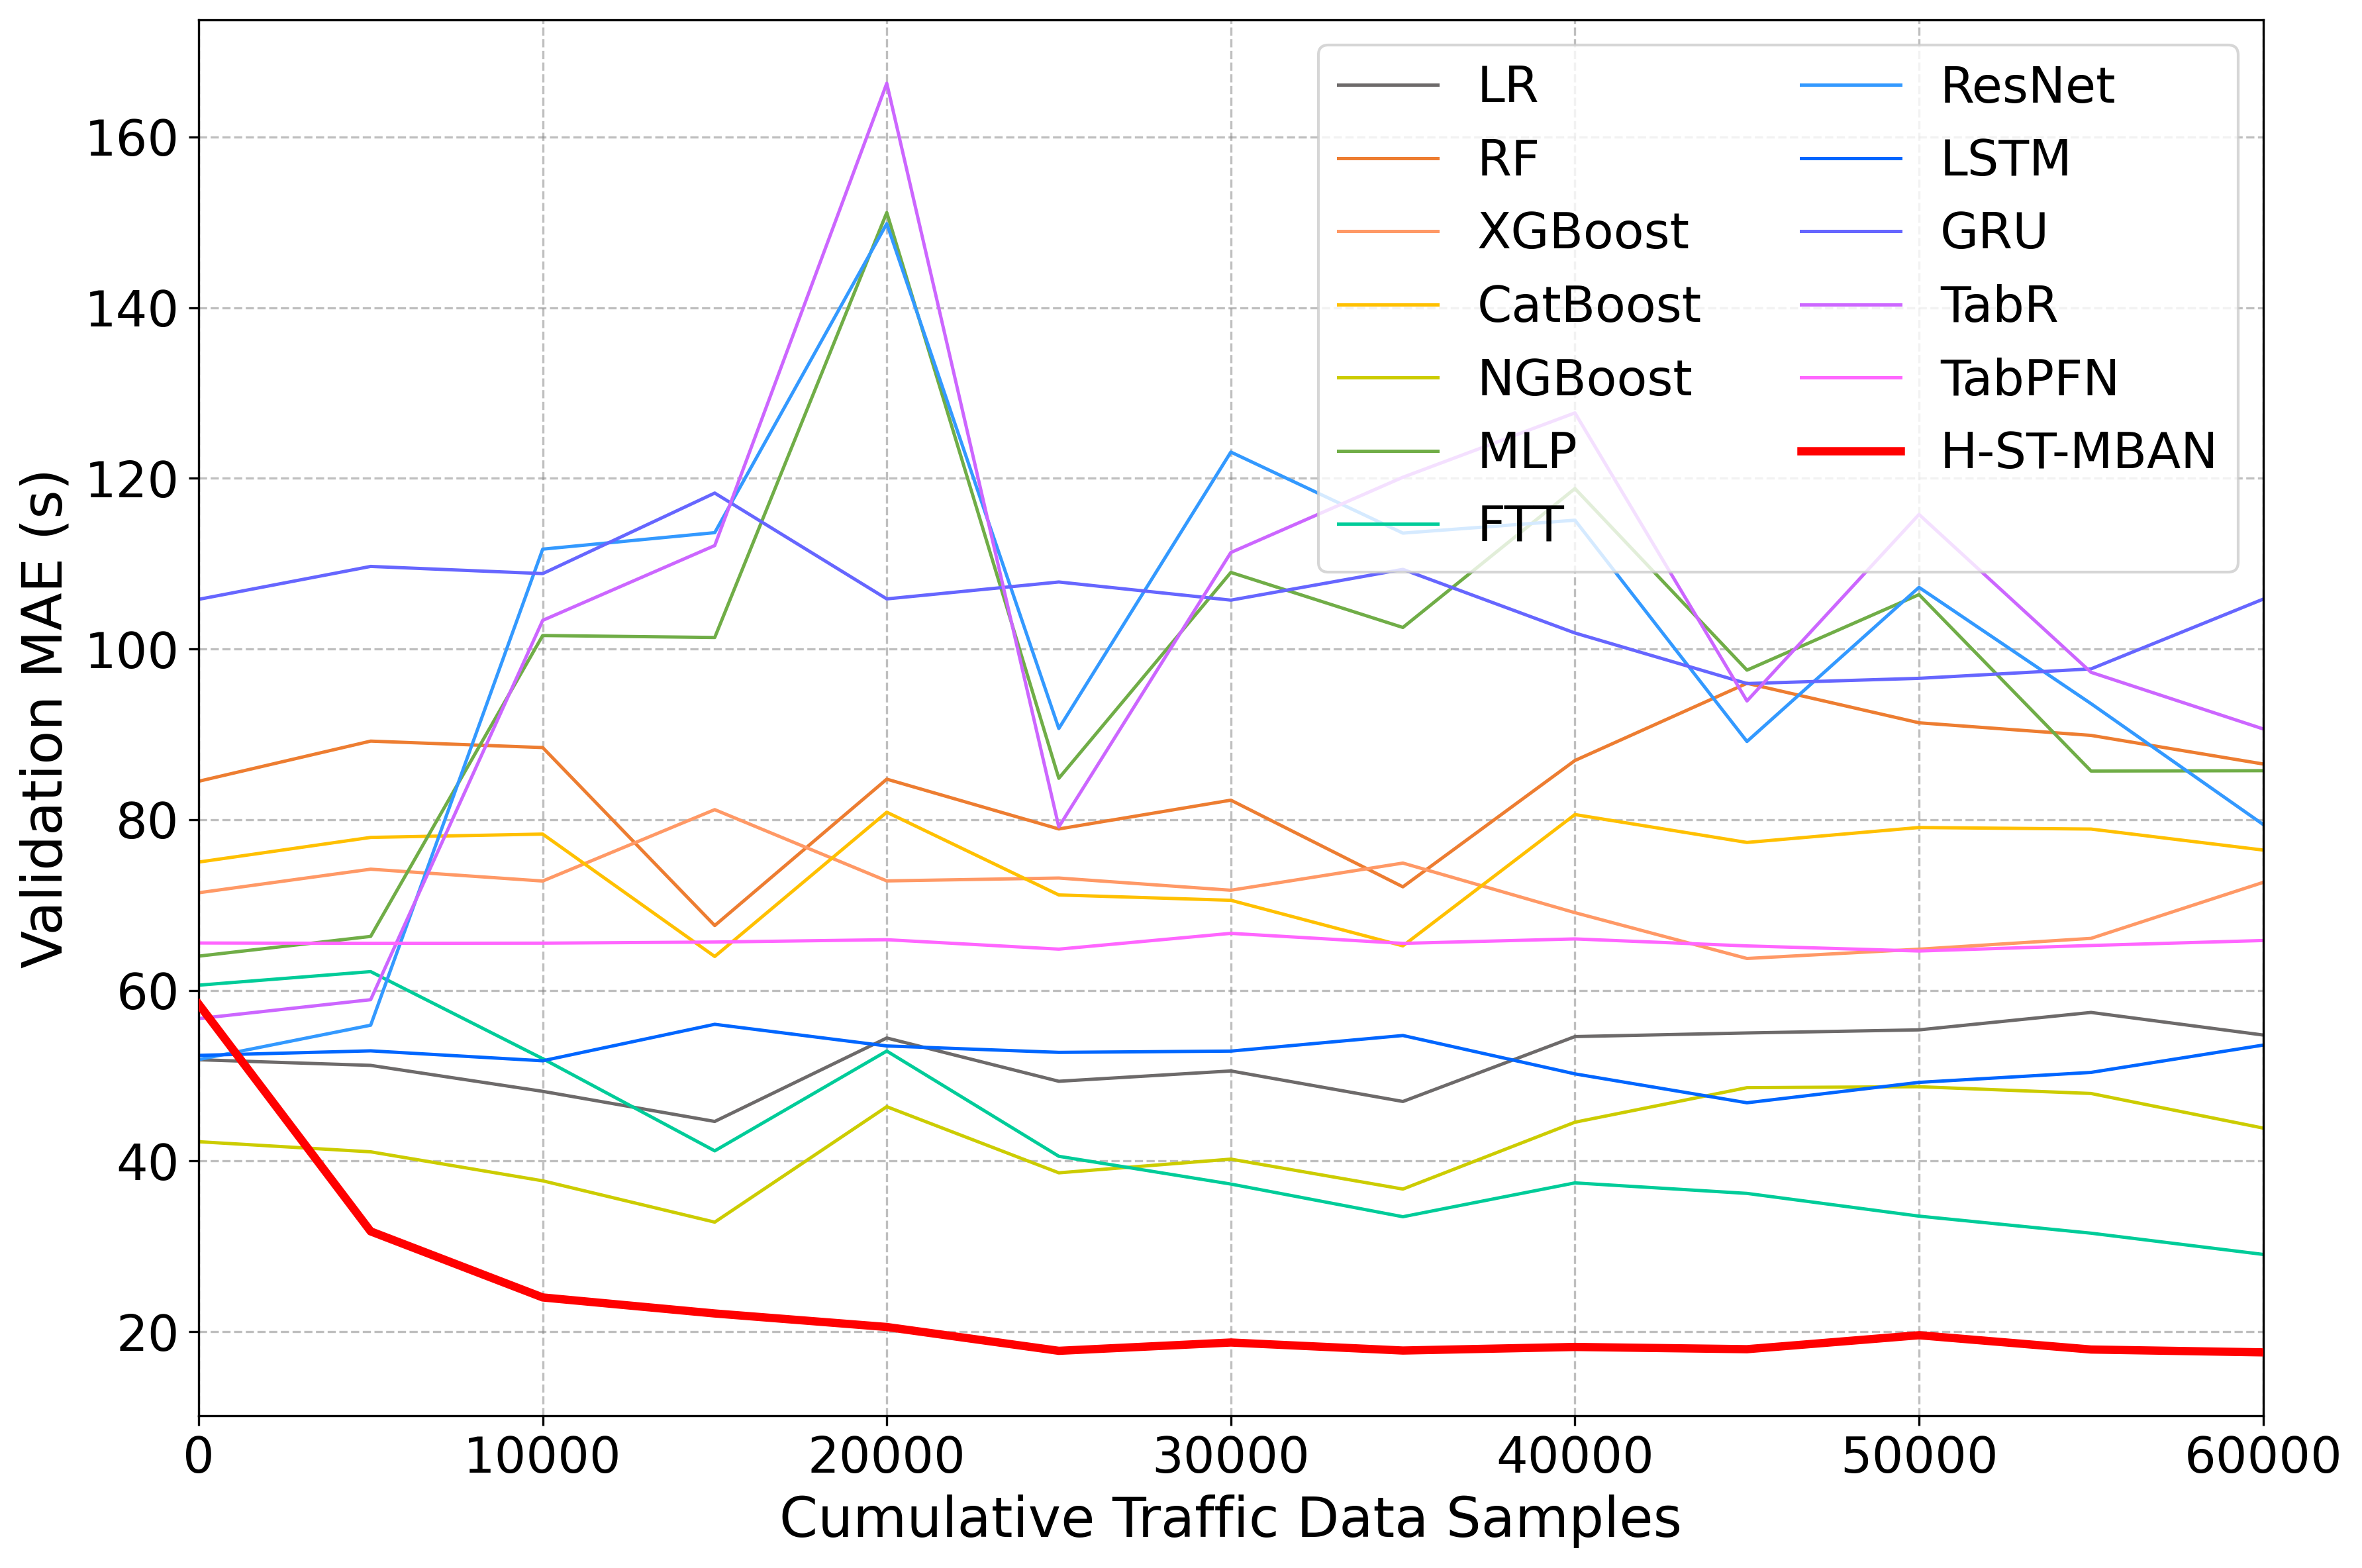
\includegraphics[width=\textwidth]{figure/G5_baseline_comparison.png}
\caption{Cumulative validation MAE comparison of H-ST-MBAN against 12 ML/NN baselines under the optimal queue size Q=5000.}
\label{fig:G5}
\end{figure*}

\begin{table}[!t]
\centering
\caption{Average MAE During Online Fine-Tuning (12 Rounds). H-ST-MBAN avoids catastrophic forgetting and achieves the lowest average MAE.}
\label{tab:finetune_accuracy}
\begin{tabular}{lccc}
\toprule
\textbf{Model} & \textbf{Global MAE (s)} & \textbf{Final MAE (s)} & \textbf{Average MAE (s) $\pm$ Std. Dev.} \\
\midrule
\textbf{H-ST-MBAN} & 58.39 & 17.58 & \textbf{20.33 $\pm$ 4.12} \\
FTT & 60.61 & 29.06 & 40.62 $\pm$ 10.02 \\
NGBoost & 42.26 & 43.86 & 42.26 $\pm$ 5.20 \\
LR & 51.87 & 54.77 & 51.87 $\pm$ 3.97 \\
LSTM & 52.38 & 53.58 & 52.06 $\pm$ 2.54 \\
TabPFN & 65.55 & 65.84 & 65.55 $\pm$ 0.55 \\
XGBoost & 71.44 & 72.65 & 71.44 $\pm$ 4.86 \\
CatBoost & 75.03 & 76.44 & 75.03 $\pm$ 5.85 \\
RF & 84.50 & 86.53 & 84.50 $\pm$ 8.15 \\
MLP & 64.01 & 85.74 & 100.91 $\pm$ 21.04 \\
ResNet & 51.89 & 79.44 & 103.58 $\pm$ 23.86 \\
GRU & 105.82 & 105.84 & 105.29 $\pm$ 6.45 \\
TabR & 56.69 & 90.64 & 106.38 $\pm$ 26.74 \\
\bottomrule
\end{tabular}
\end{table}

\subsection{G6: Cache Hit Ratio and Delay}
Figure~\ref{fig:G6} presents the average cache performance metrics. The results indicate that H-ST-MBAN achieves an average cache hit ratio of 90.70\% alongside a low average access delay of 0.1196~\text{s} and reduced wasted traffic of 17.70~\text{MB}, demonstrating competitive precaching performance compared to the 12 baseline models, which span traditional machine learning, standard deep learning, and advanced tabular models. This performance advantage stems from the model's ability to accurately predict vehicle dwell times, allowing roadside units to proactively cache content with high precision. By improving the accuracy of cache placement, the proposed approach reduces both the latency experienced by end users and the redundant network traffic caused by incorrectly cached data. On the other hand, the baseline models show lower hit ratios and increased latency, highlighting the critical importance of reliable dwell time prediction for edge caching systems. This reduction in wasted traffic is particularly valuable when backhaul capacity is leased or bandwidth-constrained, as it directly translates to lower operational costs.

\begin{figure*}[!t]
\centering
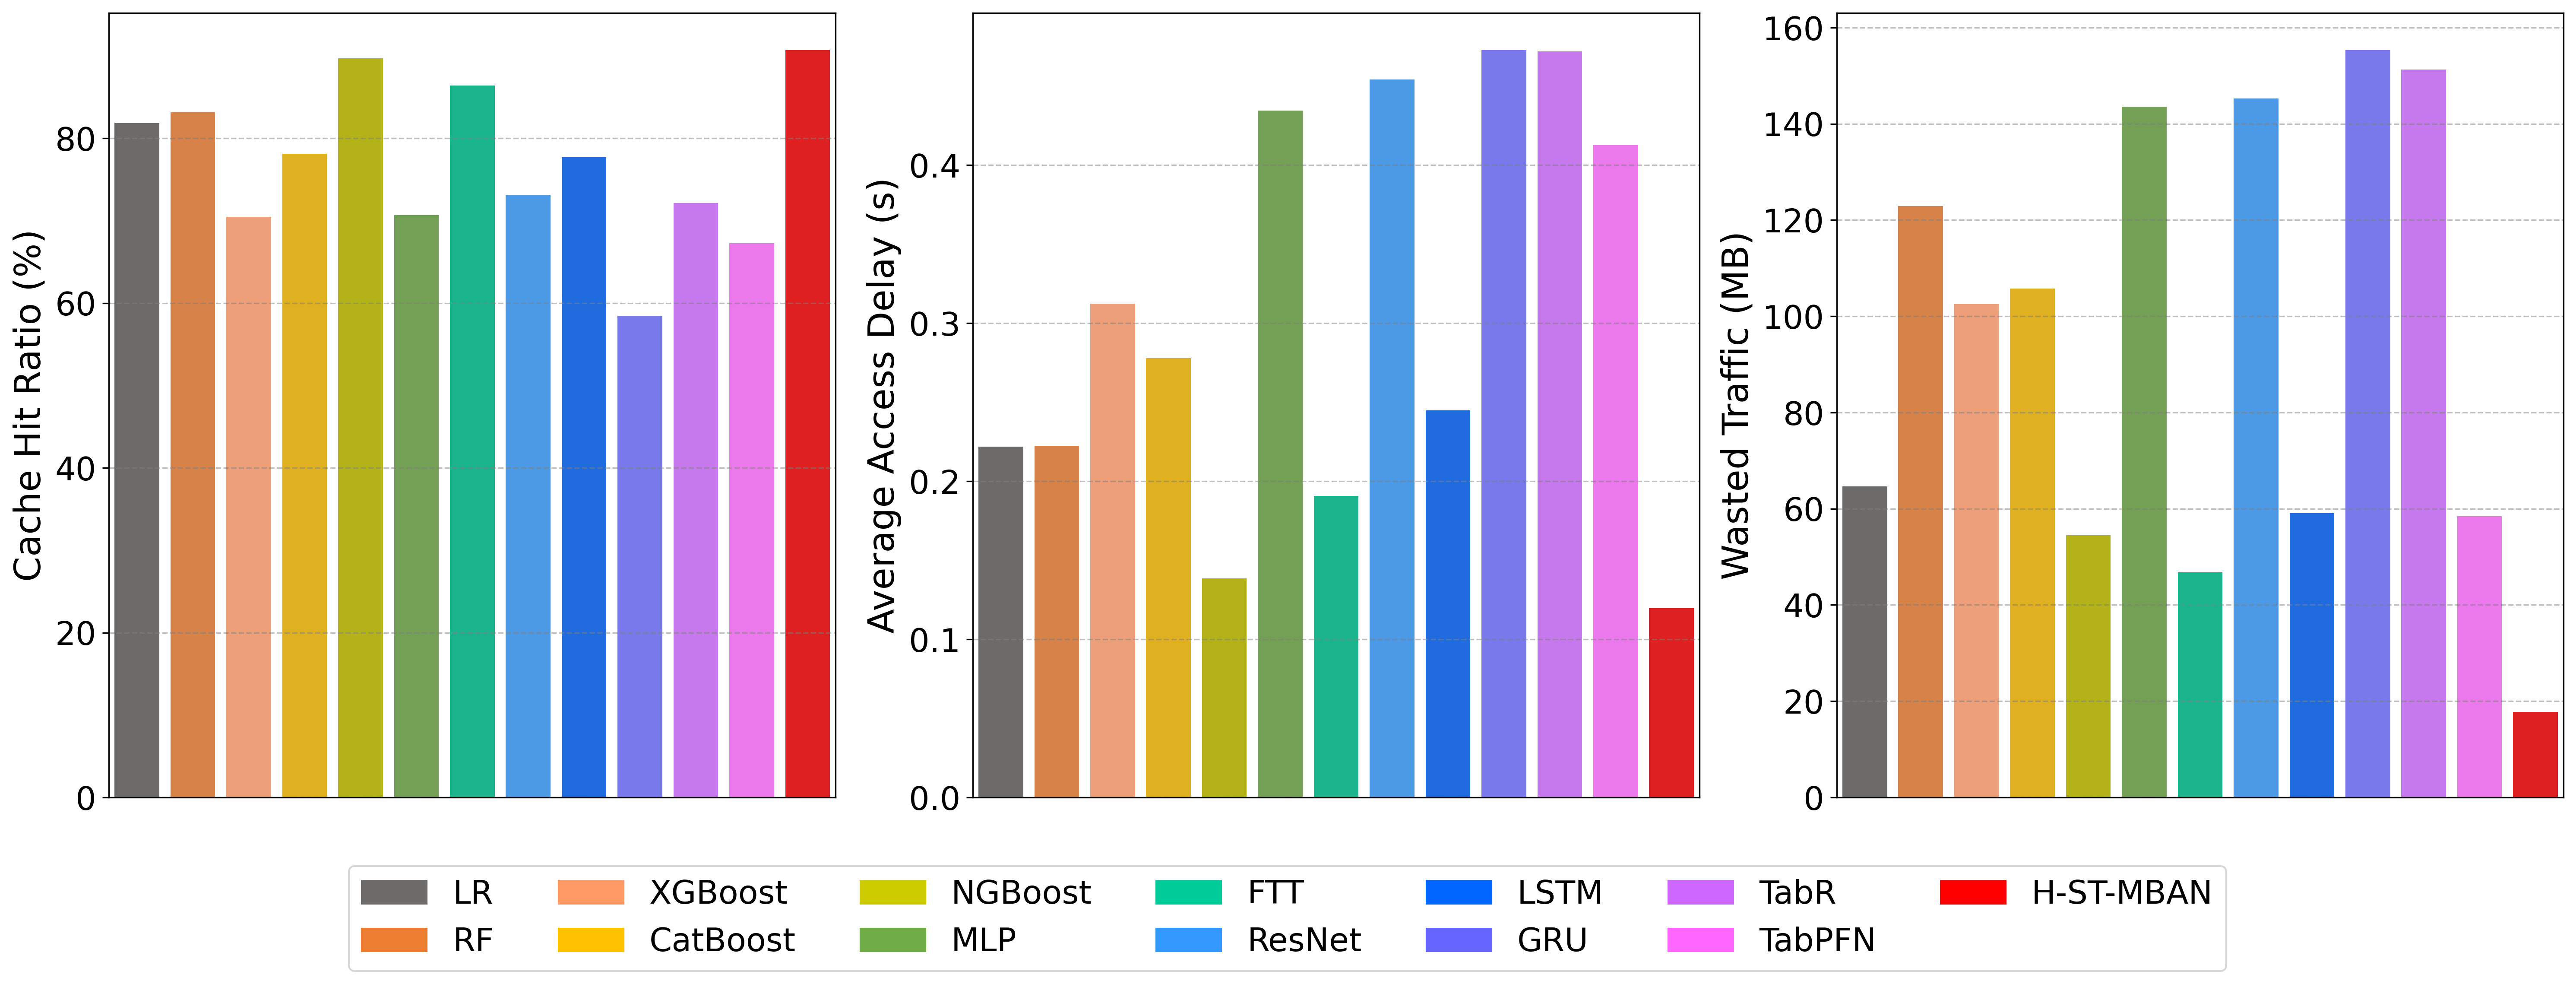
\includegraphics[width=\textwidth]{figure/G6_cache_metrics_avg.png}
\caption{G6 (Average Cache Performance Metrics): Cache hit ratio, access delay, and wasted traffic comparing H-ST-MBAN against 12 baseline models.}
\label{fig:G6}
\end{figure*}

\subsection{G7: Cache Metrics by Vehicle Density}
Figure~\ref{fig:G7} illustrates the impact of varying vehicle densities on cache performance. Specifically, in the high-density traffic interval of $(22.5, 25.0]~\text{veh/km/lane}$, H-ST-MBAN maintains a cache hit ratio of 91.64\% and low access latency, which demonstrates its operational stability. Conversely, the baseline models experience performance degradation under similar conditions. This decline in baseline performance is primarily due to their inability to capture the increasingly complex spatial queuing dynamics and inter-vehicle interactions inherent in dense traffic. The sustained efficiency of H-ST-MBAN highlights the performance of its hybrid spatio-temporal design in managing intricate congestion patterns without sacrificing predictive accuracy. This stable caching performance under high vehicle densities confirms that the network can maintain service quality even during peak traffic hours.

\begin{figure*}[!t]
\centering
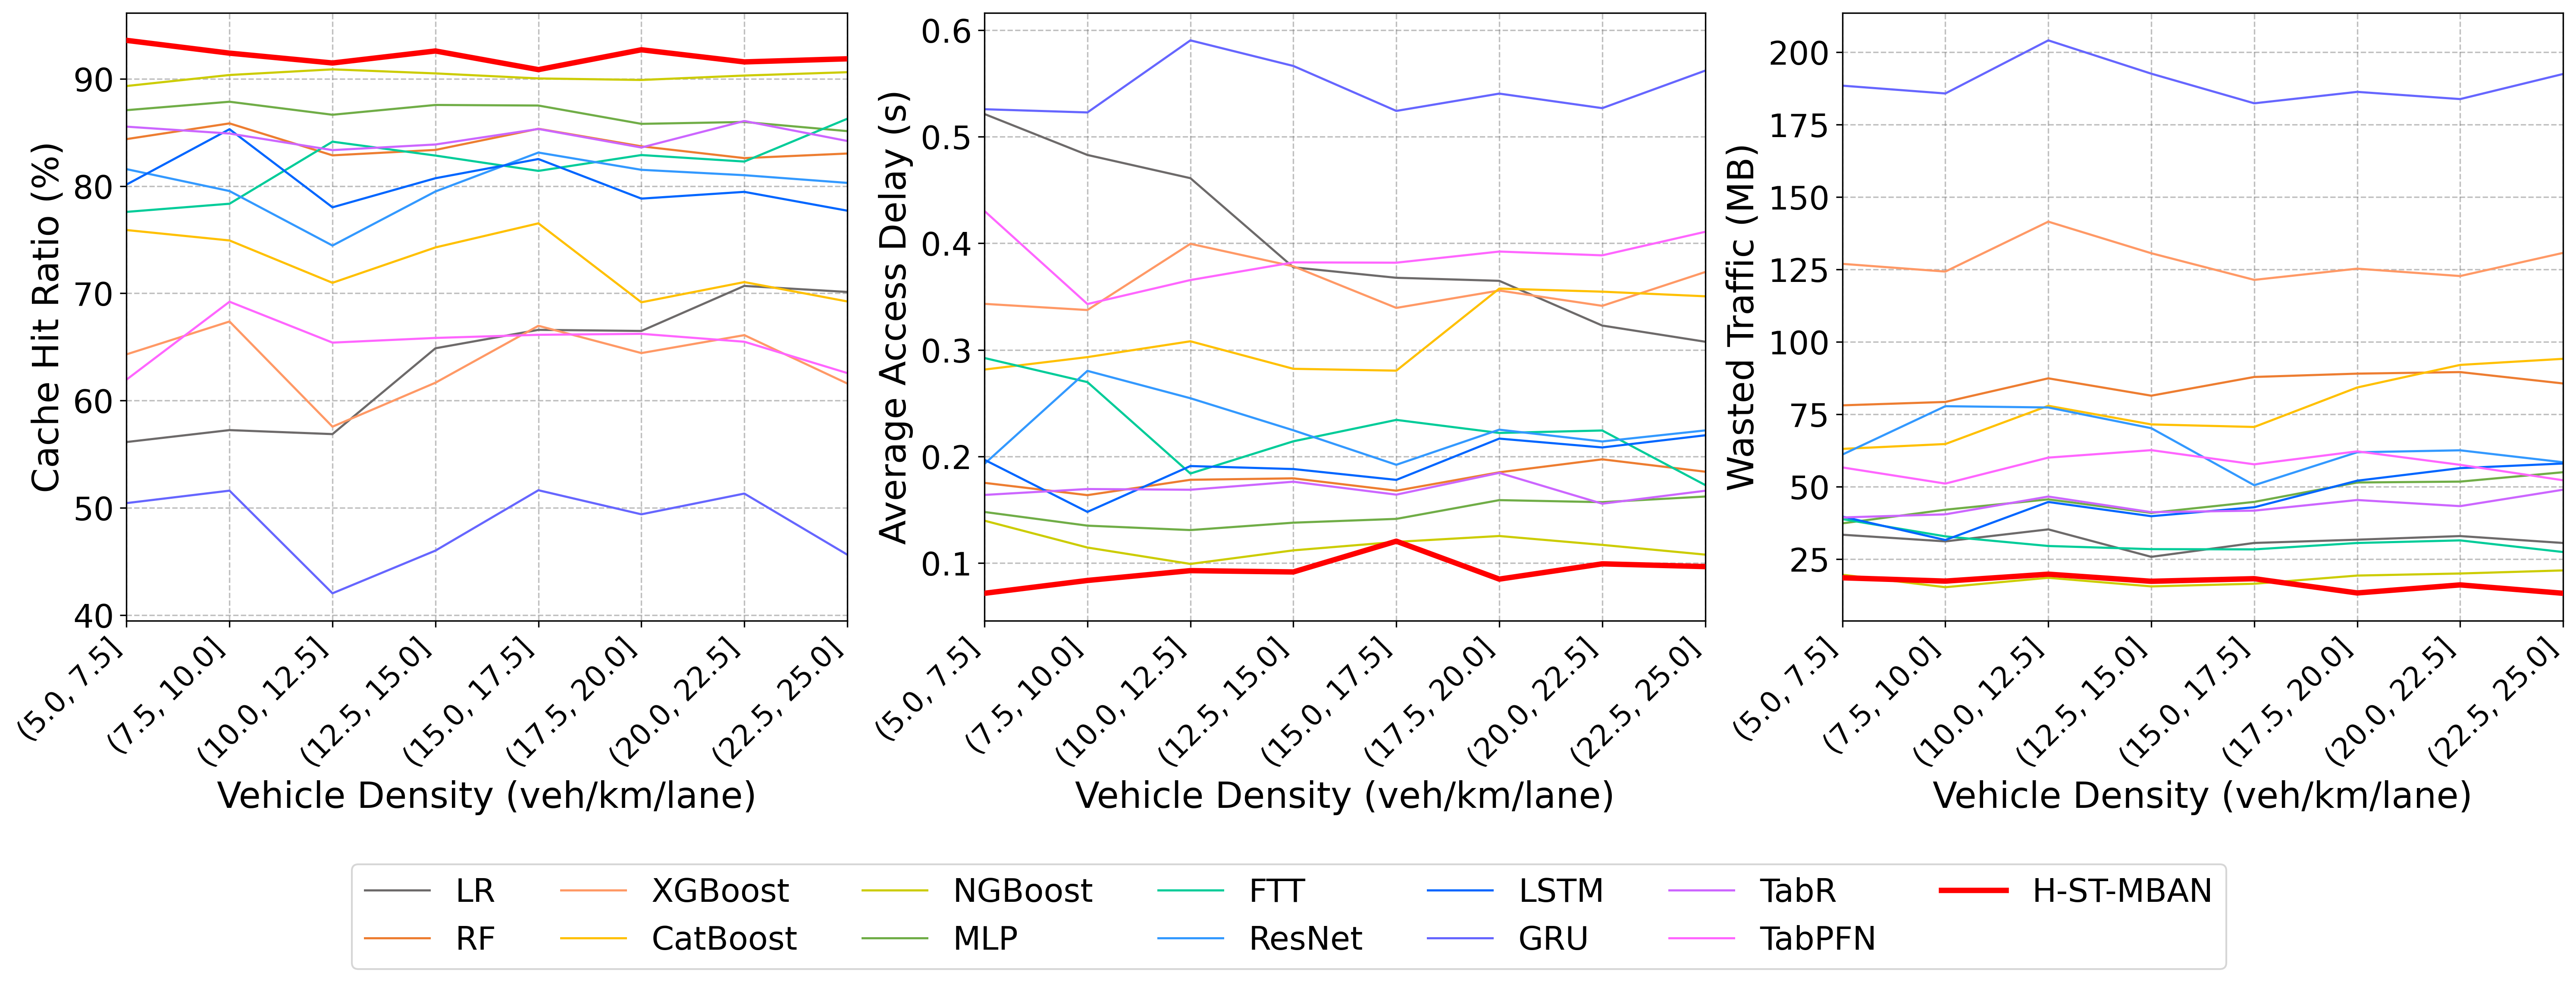
\includegraphics[width=\textwidth]{figure/G7_cache_metrics_density.png}
\caption{G7 (Cache Metrics by Vehicle Density): Cache performance under varying vehicle densities, demonstrating the stability of H-ST-MBAN against complex spatial queuing dynamics.}
\label{fig:G7}
\end{figure*}
% ============================================================
\section{Conclusion}\label{sec:conclusion}
% ============================================================
In this paper, we proposed H-ST-MBAN, a deterministic regression model for dwell-time prediction in Content-Centric Vehicular Networks.
To overcome complex traffic patterns and localized inference latency, H-ST-MBAN adopts a hybrid residual regression architecture.
By establishing an accurate XGBoost base prediction and learning the spatio-temporal residual errors through semantically partitioned branch encoders fused via multi-head self-attention, H-ST-MBAN captures complex traffic dynamics without high computational overhead.
Evaluations using the SUMO traffic simulator indicated that H-ST-MBAN achieves the lowest prediction error compared to 12 baseline models.
Ablation studies showed that the GBDT prior stream, multi-branch attention structure, and deep residual decoder all contribute to maintaining prediction accuracy and ensuring fast convergence. Ultimately, the integration of physical traffic constraints with non-linear neural mapping establishes a new methodology for decentralized edge intelligence in future intelligent transportation systems.

Network-level simulations also indicated that H-ST-MBAN supports proactive caching by reducing access delay and wasted traffic, maintaining a 91.64\% cache hit ratio under high traffic density.
When vehicle density rises, traffic congestion increases the vehicle dwell time within the intersection coverage of the road-side unit.
This extended residency duration provides the edge node with sufficient time to prefetch and cache requested content chunks, enabling the system to maintain a cache hit ratio of 91.64\% under dense traffic conditions, which exceeds the average hit ratio of 90.70\%.
Finally, theoretical hardware profiling suggested that the proposed Dual-Model fine-tuning strategy is computationally feasible on standard RSU edge devices.
This feasibility allows the predictive framework to function independently without overwhelming the V2I uplink capacity.
By keeping operations strictly localized, the proposed method circumvents centralized processing bottlenecks.
In future work, we plan to extend H-ST-MBAN by integrating federated learning across multiple RSUs, enabling collaborative adaptation to city-scale traffic anomalies without compromising vehicle privacy.

% ============================================================
\section*{Acknowledgment}
% ============================================================
This work was supported by the National Research Foundation of Korea (NRF) grant funded by the Korea government (MSIT) (No. 2022R1A2C1010121).


% ============================================================
\bibliographystyle{IEEEtran}
% ============================================================

\begin{thebibliography}{31}

\bibitem{1}
Ericsson, ``Ericsson Mobility Report,'' Ericsson, June 2026. [Online]. Available: https://www.ericsson.com/en/reports-and-papers/mobility-report/reports/june-2026

\bibitem{2}
Z. Su, Y. Hui and Q. Yang, ``The Next Generation Vehicular Networks: A Content-Centric Framework,'' IEEE Wireless Communications, vol. 24, no. 1, pp. 60--66, 2017.

\bibitem{3}
M. Wang, J. Wu, G. Li, J. Li, Q. Li and S. Wang, ``Toward mobility support for information-centric IoV in smart city using fog computing,'' 2017 IEEE International Conference on Smart Energy Grid Engineering (SEGE), Oshawa, ON, Canada, 2017, pp. 357--361.

\bibitem{4}
Y. Nam, H. Choi and E. Lee, ``Content Storage Management and Precaching Scheme in Content-Centric-Network-Based Internet of Vehicles,'' IEEE Internet of Things Journal, vol. 12, no. 9, pp. 12927--12947, 2025.

\bibitem{5}
Z. Su, Y. Hui, Q. Xu, T. Yang, J. Liu and Y. Jia, ``An Edge Caching Scheme to Distribute Content in Vehicular Networks,'' IEEE Transactions on Vehicular Technology, vol. 67, no. 6, pp. 5346--5356, 2018.

\bibitem{6}
W. Huang, T. Song, Y. Yang and Y. Zhang, ``Cluster-Based Cooperative Caching With Mobility Prediction in Vehicular Named Data Networking,'' IEEE Access, vol. 7, pp. 23442--23458, 2019.

\bibitem{7}
B. Feng, C. Feng, D. Feng, Y. Wu and X. Xia, ``Proactive Content Caching Scheme in Urban Vehicular Networks,'' IEEE Transactions on Communications, vol. 71, no. 7, pp. 4165--4180, 2023.

\bibitem{8}
J. Cheng, K. Li, Y. Liang, L. Sun, J. Yan and Y. Wu, ``Rethinking Urban Mobility Prediction: A Multivariate Time Series Forecasting Approach,'' IEEE Transactions on Intelligent Transportation Systems, vol. 26, no. 2, pp. 2543--2557, 2025.

\bibitem{9}
G. Yu, J. Wu, R. Liu, Y. He, Z. Chen and J. Pan, ``Joint Cooperative Caching and UAV Trajectory Optimization Based on Mobility Prediction in the Internet of Connected Vehicles,'' IEEE Transactions on Intelligent Transportation Systems, vol. 25, no. 11, pp. 17392--17406, 2024.

\bibitem{10}
X. Zhang, Z. Chang, T. Hu, W. Chen, X. Zhang and G. Min, ``Vehicle Selection and Resource Allocation for Federated Learning-Assisted Vehicular Network,'' IEEE Transactions on Mobile Computing, vol. 23, no. 5, pp. 3817--3829, 2024.

\bibitem{11}
R. Liu and J. Pan, ``CRS: A Privacy-Preserving Two-Layered Distributed Machine Learning Framework for IoV,'' IEEE Internet of Things Journal, vol. 11, no. 1, pp. 1080--1095, 2024.

\bibitem{12}
Zhuo Li, Yutong Chen, Deliang Liu, Xiang Li, ``Performance analysis for an enhanced architecture of IoV via Content-Centric Networking,'' \textit{EURASIP Journal on Wireless Communications and Networking}, 2017, doi: 10.1186/S13638-017-0905-4.

\bibitem{13}
Irfanullah Khan, Tiankui Zhang, Xiaogeng Xu, Siyang Shan, Adil Khan..., ``Priority-based Content Dissemination in Content Centric Vehicular Networks,'' \textit{IEEE Advanced Information Management, Communicates, Electronic and Automation Control Conference}, 2018, doi: 10.1109/IMCEC.2018.8469332.

\bibitem{14}
Sajjad Ahmad Khan, Huhnkuk Lim, Shehzad Ashraf Chaudhry, ``Adaptive Data Forwarding Scheme for Diverse Infotainment Services in Vehicular Named Data Networking,'' \textit{IEEE Transactions on Vehicular Technology}, 2025, doi: 10.1109/TVT.2024.3524122.

\bibitem{15}
Huhnkuk Lim, ``Toward Infotainment Services in Vehicular Named Data Networking: A Comprehensive Framework Design and Its Realization,'' \textit{IEEE transactions on intelligent transportation systems (Print)}, 2025, doi: 10.1109/TITS.2024.3489574.

\bibitem{16}
Azan Khan, Basharat Hussain, Muhammad F. Islam, M. M. A. Dabel, Ali Kashif Bashir, ``Optimizing Content Cache With Vehicular Edge Computing: A Deep Federated Learning-Based Novel Predictive Study,'' \textit{IEEE transactions on consumer electronics}, 2025, doi: 10.1109/TCE.2025.3571029.

\bibitem{17}
Tengfei Cao, Ni Zhang, Xiaoying Wang, Jianqiang Huang, ``Mobility-Aware Cooperative Caching in Vehicular Edge Computing Based on Federated Distillation and Deep Reinforcement Learning,'' \textit{IEEE Transactions on Network Science and Engineering}, 2025, doi: 10.1109/TNSE.2025.3571902.

\bibitem{18}
Yali Wang, Shouhao Li, ``Federated Learning-based Vehicle Edge Caching Optimization Strategy,'' \textit{2025 IEEE 6th International Conference on Pattern Recognition and Machine Learning (PRML)}, 2025, doi: 10.1109/PRML66062.2025.11160265.

\bibitem{19}
Yaqin Xie, Cheng Zhou, Zhongyu Liu, Yu Zhang, Jianyue Zhu..., ``Research on Cache Placement Optimization and Popularity-Based Content Prefetching Strategy in LEO Satellite Networks,'' \textit{IEEE Transactions on Green Communications and Networking}, 2026, doi: 10.1109/TGCN.2025.3570489.

\bibitem{20}
Nyothiri Aung, Sahraoui Dhelim, L. Chen, Abderrahmane Lakas, Wenyin Zhang..., ``VeSoNet: Traffic-Aware Content Caching for Vehicular Social Networks Using Deep Reinforcement Learning,'' \textit{IEEE transactions on intelligent transportation systems (Print)}, 2023, doi: 10.1109/TITS.2023.3250320.

\bibitem{21}
Kai Jiang, Yue Cao, Yujie Song, Huan Zhou, Shaohua Wan..., ``Asynchronous Federated and Reinforcement Learning for Mobility-Aware Edge Caching in IoV,'' \textit{IEEE Internet of Things Journal}, 2024, doi: 10.1109/JIOT.2023.3349255.

\bibitem{22}
Zhoufan Liao, Pang Liu, Bin Zheng, Xiaoyong Tang, ``Context-Aware Proactive Edge Caching for Vehicular Edge Computing Based on Asynchronous Federated Learning,'' \textit{IEEE Internet of Things Journal}, 2025, doi: 10.1109/JIOT.2025.3552682.

\bibitem{23}
Chenglong Wang, Jun Peng, Lin Cai, Weirong Liu, Ziyu Zhao..., ``Mobility and Context-Aware Precaching Strategy Using Spatial-Temporal Informer for Vehicular Service,'' \textit{IEEE Internet of Things Journal}, 2025, doi: 10.1109/JIOT.2025.3530699.

\bibitem{24}
Qin Yang, Sang-Jo Yoo, ``Hierarchical Reinforcement Learning-Based Routing Algorithm With Grouped RSU in Urban VANETs,'' \textit{IEEE transactions on intelligent transportation systems (Print)}, 2024, doi: 10.1109/TITS.2024.3353258.

\bibitem{25}
G. R. Gopal, Jie Chen, W. Hillery, Jun Tan, Serdar Özen..., ``Wireless Channel Scenario Identification Using Convolutional Neural Networks,'' \textit{IEEE Vehicular Technology Conference}, 2023, doi: 10.1109/VTC2023-Spring57618.2023.10200552.

\bibitem{26}
M. Hasan, Nusrat Jahan, Mohd Zakree Ahmad Nazri, S. Islam, Muhammad Attique Khan..., ``Federated Learning for Computational Offloading and Resource Management of Vehicular Edge Computing in 6G-V2X Network,'' \textit{IEEE transactions on consumer electronics}, 2024, doi: 10.1109/TCE.2024.3357530.

\bibitem{27}
Bo Xu, Haitao Zhao, Haotong Cao, Xiaozhen Lu, Hongbo Zhu, ``Joint Contract Design and Task Reorganization for Semi-Decentralized Federated Edge Learning in Vehicular Networks,'' \textit{IEEE Transactions on Vehicular Technology}, 2024, doi: 10.1109/TVT.2024.3364515.

\bibitem{28}
Soohyun Park, C. Park, Soyi Jung, Minseok Choi, Joongheon Kim, ``Age-of-Information Aware Caching and Delivery for Infrastructure-Assisted Connected Vehicles,'' \textit{IEEE Transactions on Vehicular Technology}, 2024, doi: 10.1109/TVT.2024.3384952.

\bibitem{29}
Jie Hu, Li Shen, and Gang Sun, ``Squeeze-and-Excitation Networks,'' in \textit{Proceedings of the IEEE Conference on Computer Vision and Pattern Recognition (CVPR)}, 2018, pp. 7132--7141.

\bibitem{30}
Ashish Vaswani, Noam Shazeer, Niki Parmar, Jakob Uszkoreit, Llion Jones, Aidan N. Gomez, Lukasz Kaiser, and Illia Polosukhin, ``Attention Is All You Need,'' in \textit{Advances in Neural Information Processing Systems}, 2017, pp. 5998--6008.

\bibitem{31}
Intelligent Transportation Systems Joint Program Office, ``ITS Standards Program: Strategic Plan 2021--2026,'' \textit{U.S. Department of Transportation}, 2021.

\end{thebibliography}

\end{document}
